\documentclass[a4paper,12pt, oneside]{article}

\title{\textbf{L'impatto del Codec AV1 sull'industria della visualizzazione online} \\ \large A.A 2023/2024 \\ Elaborato di Crittografia}
\author{Gabos Norbert \\ 0000970451 \\ tiberiunorbert.gabos@studio.unibo.it }
\date{}

\usepackage[T1]{fontenc}
\usepackage[utf8]{inputenc}
\usepackage[italian]{babel}
\pagestyle{plain}
\usepackage{graphicx}
\usepackage{hyperref}   % serve per i link
\hypersetup{
    colorlinks=true,
    linkcolor=black,
    filecolor=magenta,      
    urlcolor=cyan,
}   % serve per i link
\graphicspath{{images/}}

\usepackage{multicol}   % permette di creare liste su più colonne
\usepackage{enumitem}   % permette di "poter" togliere il bullet all'inizio di un itemize

\begin{document}

\maketitle

\newpage
\tableofcontents{}
\newpage

\section{Introduzione}
Con l'avvento dei computer e la crescente digitalizzazione dei media, è emersa la necessità di
trovare soluzioni efficaci per rappresentare e archiviare i video all'interno dei sistemi
informatici. Questo processo ha comportato la trasformazione dei tradizionali filmati in una
forma compatibile con il mondo digitale, dove ogni istante del video è rappresentato da una
sequenza di immagini statiche, comunemente note come frame. Ogni frame, a sua volta, è
composto da una matrice di pixel, gli elementi fondamentali che compongono l'immagine, ognuno
dei quali è definito da una terna di colori \textbf{RGB} (Red, Green, Blue) e da una profondità
di colore che varia generalmente tra 0 e 255.

Questo approccio ha permesso di preservare la qualità visiva dei contenuti video e di renderli
compatibili con le capacità di elaborazione dei computer. Tuttavia, la mera rappresentazione
dei video in questo modo ha portato ad un'elevata quantità di dati da gestire ed archiviare
comportando sfide significative in termini di spazio di archiviazione e larghezza di banda.
Per esempio un banale video da 10 minuti in 1080p a 30 fotogrammi al secondo pesa
all'incirca 111 GB.
\noindent
\\\\Peso\_video = Risoluzione × Fotogrammi\_al\_secondo × Durata × Profondità\_colore\\

Nei primi anni '80, con il crescente bisogno di gestire file video in un contesto di limitate
capacità di archiviazione, si svilupparono i primi \textbf{codec} video. Questi non solo consentivano
la compressione dei file video, ma anche la decodifica. Questo rappresentava una soluzione
importante, poiché i dispositivi dell'epoca potevano immagazzinare solo una quantità limitata
di dati, mentre le esigenze di qualità video e il numero di dispositivi produttori di contenuti
multimediali aumentavano costantemente.
Per affrontare queste sfide e ottimizzare l'archiviazione e la trasmissione dei video
digitali, sono stati sviluppati una serie di algoritmi e standard di compressione video.
Esistono due approcci principali alla compressione video: la compressione \textbf{lossless} e
la compressione \textbf{lossy}. La compressione lossless, ad esempio con algoritmi come
\textbf{Huffyuv} e \textbf{Lagarith}, mira a ridurre le dimensioni del file senza perdita di
qualità, mantenendo ogni singolo dato originale. D'altro canto, la compressione lossy
sacrifica una certa quantità di qualità visiva per raggiungere una maggiore compressione dei
dati, consentendo una gestione più efficiente delle risorse di archiviazione e una
trasmissione più rapida attraverso le reti digitali.

In questa relazione, esploreremo l'evoluzione della compressione video lossy, partendo dal
contesto della sua necessità fino alla discussione di algoritmi più recenti e avanzati come il
Codec AV1. Analizzeremo come questi algoritmi hanno rivoluzionato il modo in cui i video
vengono elaborati, archiviati e trasmessi sui mezzi digitali, con un focus particolare sugli
impatti e le potenzialità di tali innovazioni nell'industria multimediale moderna.

\section{I primi passi}
\subsection{H.261}
Nel 1988 nasce il codec H261 che è stato il primo algoritmo di compressione video ad utilizzare
in modo efficiente degli algoritmo di \textbf{intraframe} e \textbf{interframe}, che sono
spiegati nel capitolo successivo, ed è responsabile dell'introduzione della codifica video
ibrida basata su blocchi, che è ancora utilizzata oggi in molti standard video.
\\\\Prima di proseguire, visto che non parliamo più dei video come una matrice di pixel, ma più di
un flusso di dati, bisogna introdurre il concetto di bitrate.
Il \textbf{bitrate} è una misura della velocità di trasmissione dei dati in un file multimediale,
come un video o un brano audio. Rappresenta quanti dati vengono trasmessi o elaborati in un
determinato intervallo di tempo espresso in \textbf{bit/s}. In generale, a parità di tecnologie
utilizzate per la compressione, più il bitrate di un contenuto è elevato e più la sua qualità
sarà maggiore al costo di un peso più elevato. Vedi Figura~\ref{fig:confronto_bitrate}.

\begin{figure}[h]
    \centering
    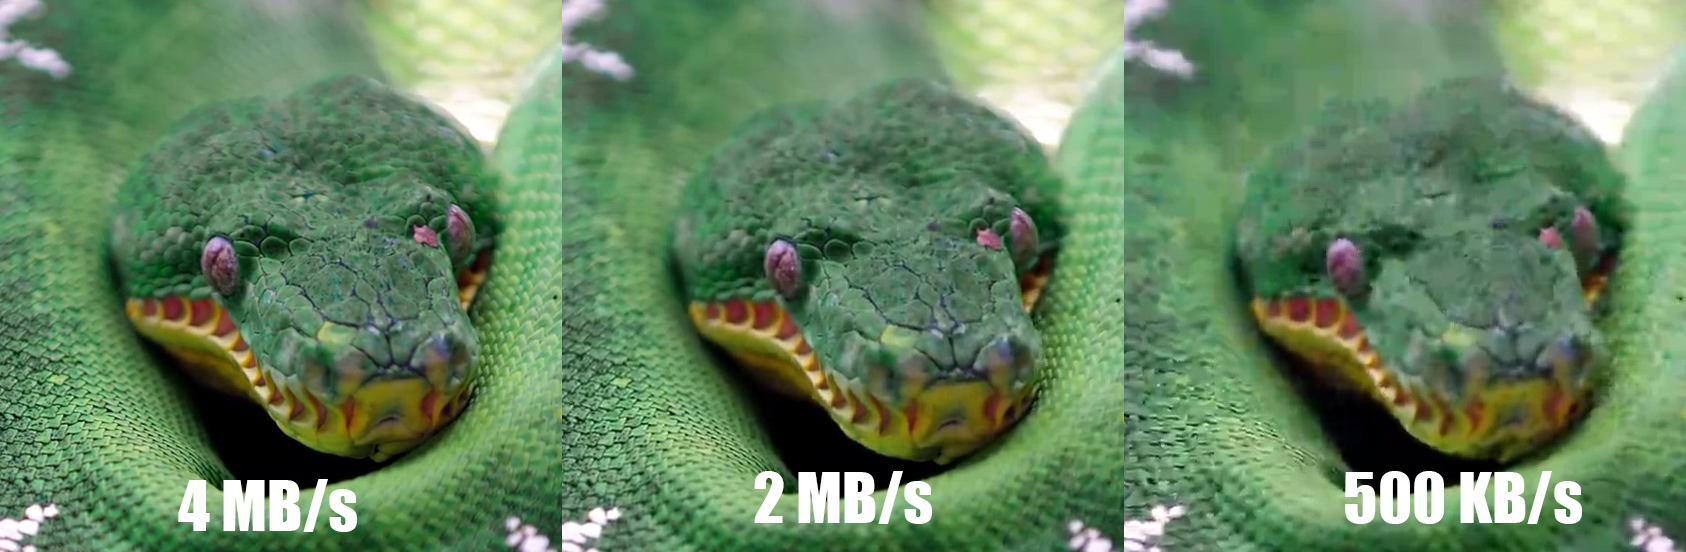
\includegraphics[width=1\textwidth]{images/confronto-bitrate.png}
    \caption{L'immagine mette a confronto 3 frame presi allo stesso istante da un video compresso con 3 valori di bitrate differenti.}
    \label{fig:confronto_bitrate}
\end{figure}

\noindent Un aspetto sorprendente di questo algoritmo è che per rilevare una diminuzione nella qualità
del video, è necessario ridurre significativamente il bitrate. Per fare un confronto con l'esempio di
prima del video da 10 minuti, utilizzando questo codec potremmo ridurre nettamente la dimensione del
file anche di 300 volte. Usando un bitrate che varia dai 5-10 Mb/s, quindi un bit rate elevato per
questa risoluzione che ci permette di mantenere un'ottima qualità, il file compresso avrebbe una
dimensione dai 375 ai 750 MB.

\subsection{Luma \& Chroma}
Quando si rappresenta un video o un'immagine in generale, la prima idea che viene in mente è quella di
rappresentare ogni pixel come una terna di informazioni, in cui ciascun componente indica l'intensità
di uno dei tre colori primari (R - rosso, G - verde, B - blu), come si può notare dalla
figura~\ref{fig:n_rgb}. In questo modo, è possibile riprodurre quasi tutti i colori esistenti (o
comunque percepibili dall'occhio umano). Inoltre, questa tecnica consente di visualizzare direttamente
le immagini sui monitor senza necessità di conversione, poiché questi dispositivi utilizzano già questo
metodo per proiettare le immagini sullo schermo.

\begin{figure}[h]
    \centering
    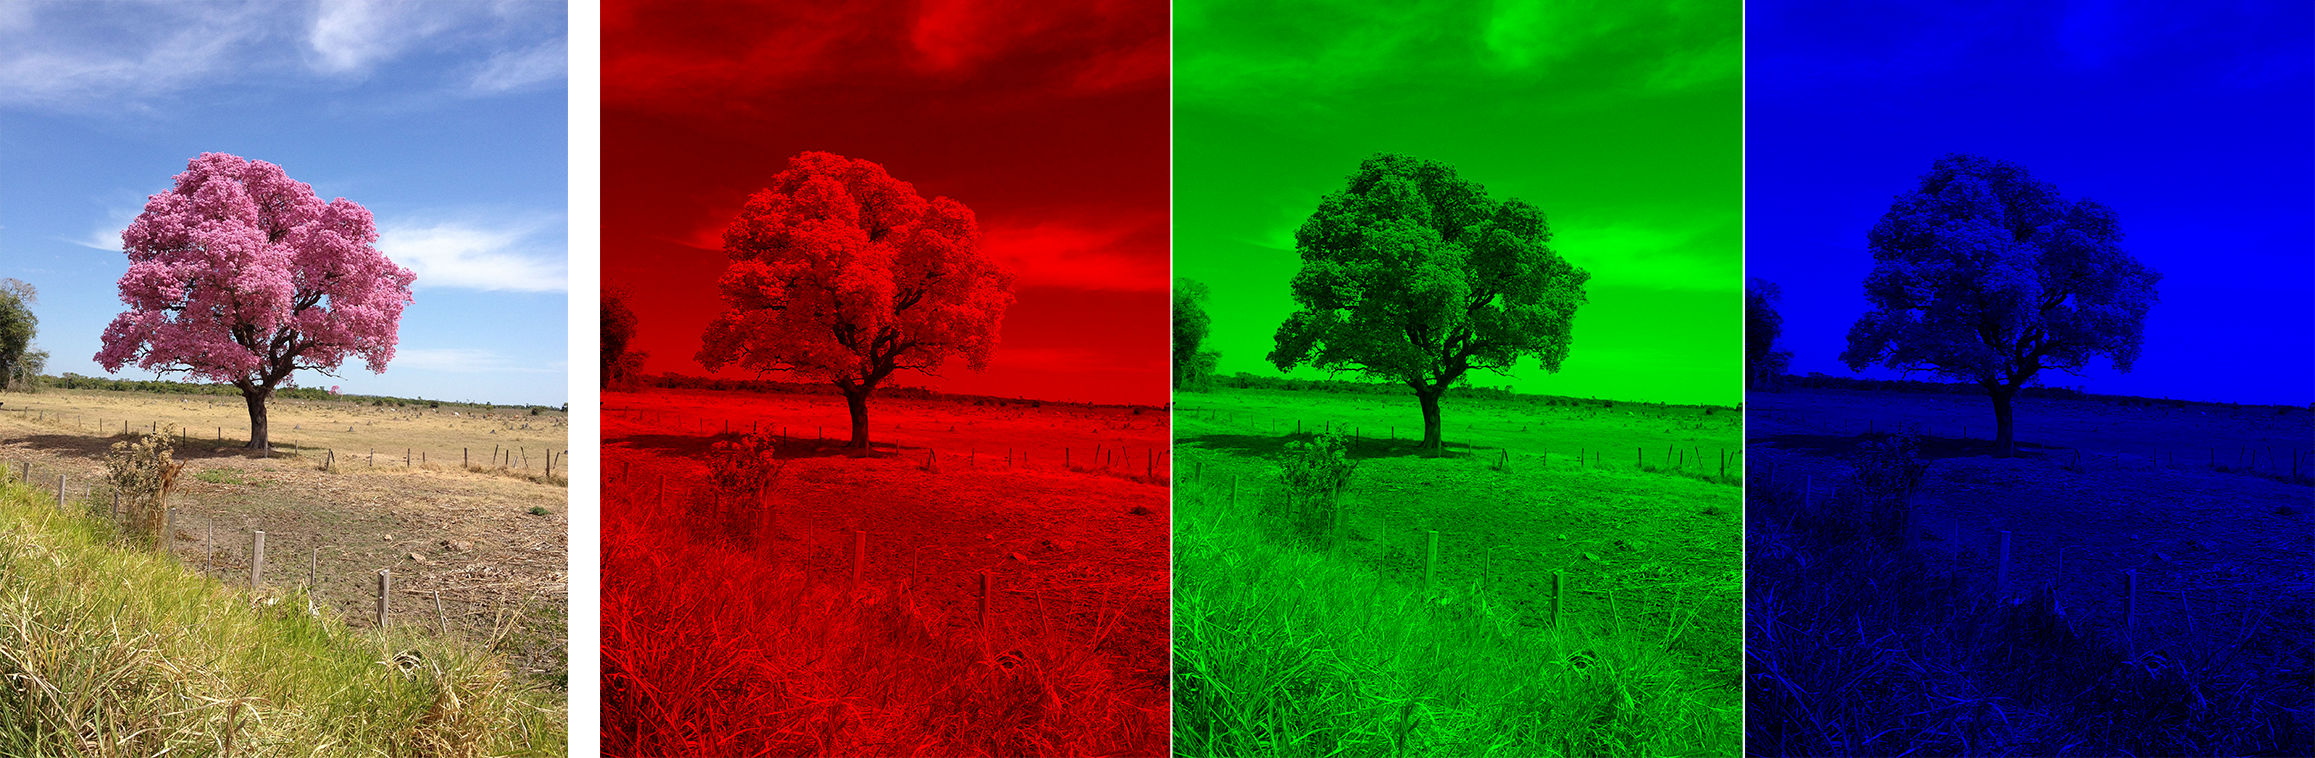
\includegraphics[width=1\textwidth]{images/n-rgb.png}
    \caption{Rappresentazione di come un'immagine viene divisa nelle sue 3 componenti di colore rosso-verde-blu.}
    \label{fig:n_rgb}
\end{figure}

Questo approccio, sebbene semplice e intuitivo, non è la scelta migliore per la codifica poiché non
offre particolari vantaggi in questo contesto. Pertanto, è stato sviluppato un nuovo metodo che
suddivide l'immagine in componenti in modo tale che alcune contengano informazioni cruciali, mentre
altre contengano dettagli meno importanti. Questo permette di mantenere la qualità visiva anche se
alcune informazioni vengono compresse o scartate completamente, poiché la perdita di dettaglio non
risulta percepibile.

Quindi è stato sviluppato un nuovo spazio di colori chiamato YCbCr, chiamato così dalla combinazione
delle sue componenti. Esso, come lo spazio RGB si divide in 3 componenti (vedi Figura~\ref{fig:n_YCbCr}):

\begin{itemize}
    \item \textbf{Luma (Y)}: La luminanza rappresenta la componente di luminosità del segnale video.
    È responsabile della rappresentazione del livello di luminosità dell'immagine senza tener conto
    del colore. In pratica, la Luma è ciò che determina la nitidezza e la luminosità dell'immagine.
    \item \textbf{Chroma (Cb e Cr)}: La crominanza, o Chroma, rappresenta la componente del colore
    del segnale video. Contrariamente alla Luma, la crominanza descrive le informazioni sul colore
    senza influire sulla luminosità. È composta da due componenti, Cb (blu) e Cr (rosso), che
    rappresentano la differenza tra la componente di colore e la luminanza.
\end{itemize}

\begin{figure}[h]
    \centering
    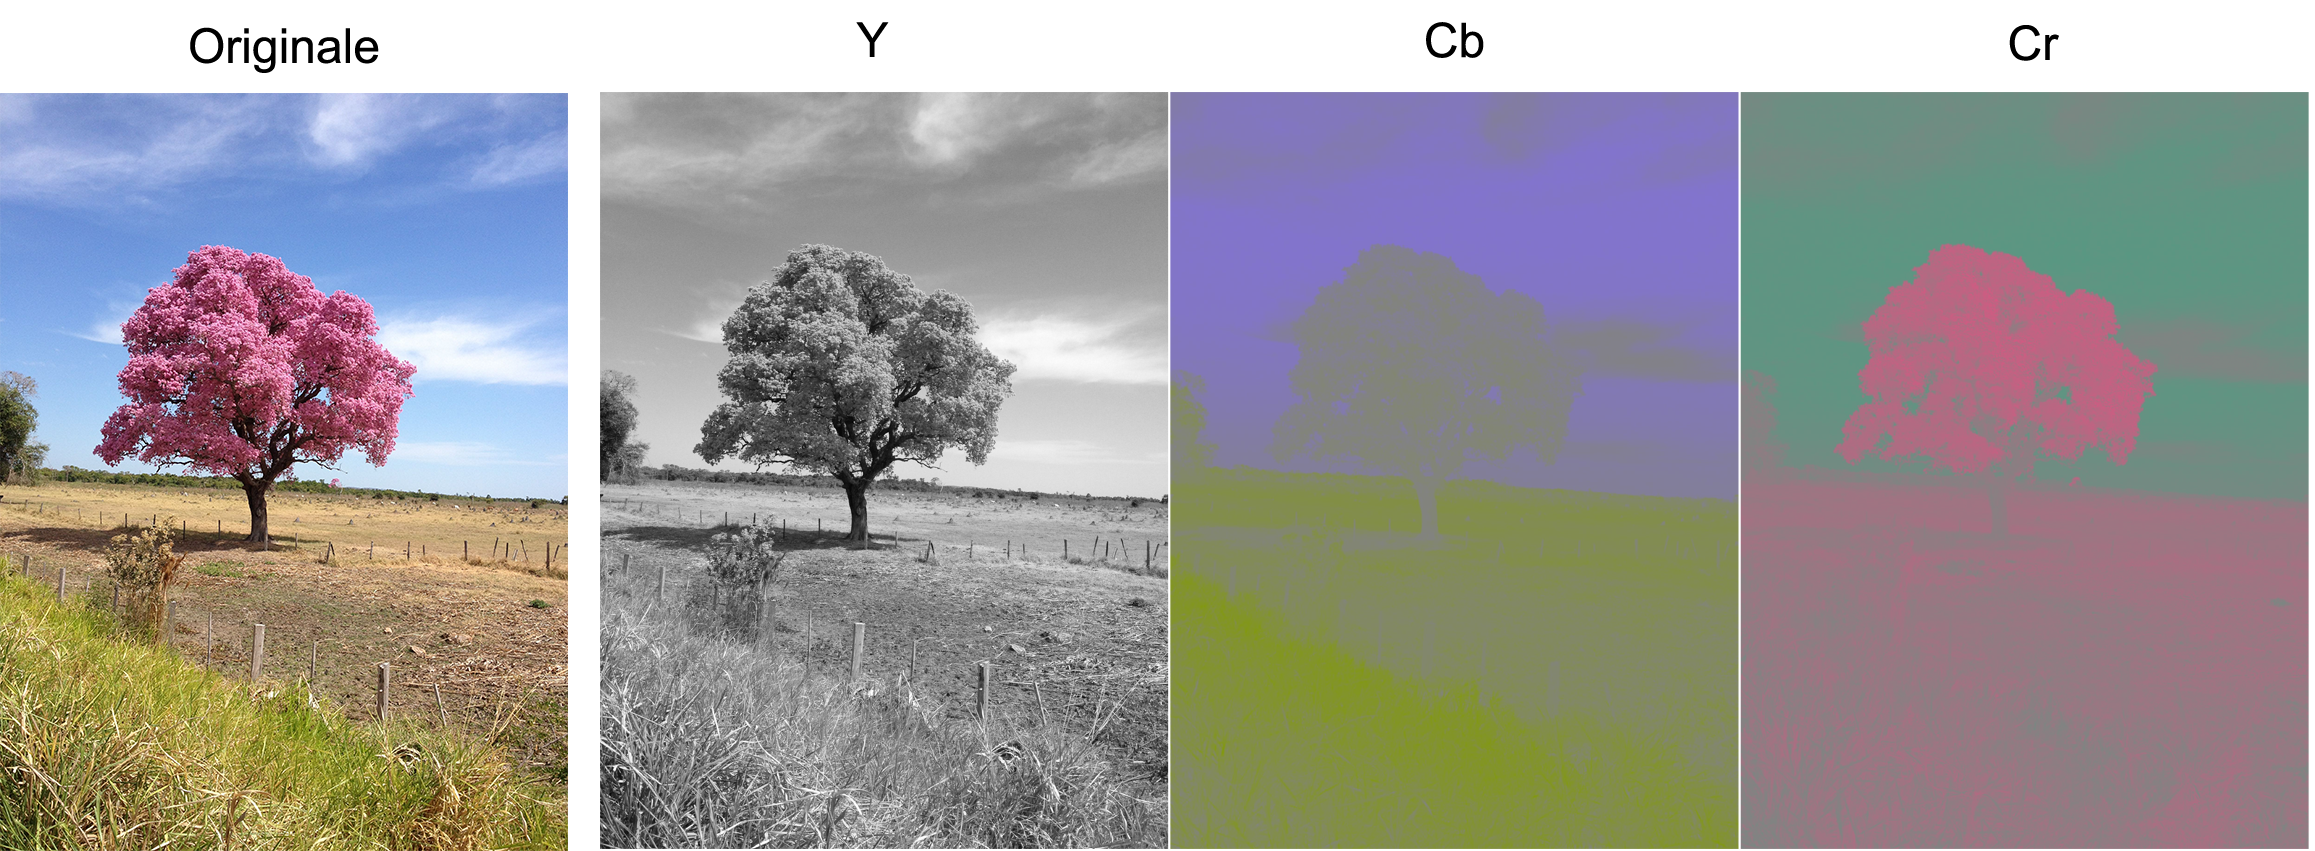
\includegraphics[width=1\textwidth]{images/n-YCbCr.png}
    \caption{Rappresentazione di come un'immagine viene divisa nelle sue 3 componenti Luma e le due
    Chroma.}
    \label{fig:n_YCbCr}
\end{figure}

Rappresentando un'immagine mediante questo spazio di colore, si è notato che la componente Luma è
nettamente più importante rispetto alle componenti Chroma. Anche alterando significativamente le
Chroma, infatti, le differenze risultano quasi impercettibili, mentre anche piccole variazioni
della componente Luma producono cambiamenti sensibilmente visibili.
Grazie a questo accorgimento si è deciso di comprimere le due componenti Chroma riducendo di molto
la dimensione dell'immagine. Ad esempio riducendo la loro dimensione di due volte, si ottiene già
una compressione del 50\% dell'immagine e dal punto di vista visivo non ci sono quasi differenze.

\section{Tecnologie attuali}
Dopo l'introduzione dell'H.261, che rappresenta uno dei primi codec video utilizzati per la compressione
digitale, l'evoluzione tecnologica ha portato allo sviluppo di codec sempre più efficienti e sofisticati.
Tra questi, l'H.264 creato nel 2003 e l'H.265 creato nel 2013 hanno segnato tappe fondamentali nel campo
della compressione video. Ovviamente questi non sono gli unici codec efficienti che sono stati creati nel
trentennio successivo all'H261, ma in questo report si parlerà principalmente di questi in quanto non
solo sono i due codec che hanno rivoluzionato maggiormente l'industria, ma sono anche i due codec più
usati ad oggi.

\subsection{H.264/AVC}
Il formato H.264 è stato introdotto nel 2003 e appartiene alla serie H.26X. Il suo obiettivo principale
è quello di comprimere ulteriormente i file video senza compromettere la qualità visiva. Questa
tecnologia consente di ottenere file video più leggeri mantenendo comunque un'elevata qualità
dell'immagine. In alternativa, è possibile mantenere le stesse dimensioni dei file video ma migliorare
la qualità visiva. Questo codec sarà fondamentale anche in futuro con l'espansione dei servizi di
streaming in tempo reale. Ciò permetterà alle aziende di risparmiare sui costi delle infrastrutture
per l'archiviazione e la trasmissione dei dati via rete, e offrirà agli utenti finali con connessioni
internet di scarsa qualità la possibilità di fruire di questi servizi.

Nonostante siano trascorsi più di 20 anni dalla creazione del formato H.264, merita comunque attenzione
in virtù del suo status di standard rivoluzionario nella codifica video. Nel settembre 2019, ha
raggiunto un notevole 91\% di adozione tra gli sviluppatori nel settore video, confermandosi così come
un pilastro fondamentale della tecnologia di compressione video. Inoltre, alcune delle tecnologie
adottate da questo codec saranno cruciali per comprendere meglio il funzionamento dei codec successivi.

\subsubsection{Slices}
Una slice è una porzione sequenziale di dati all'interno di un frame video. Questa porzione è suddivisa
in unità più piccole chiamate macroblock. La divisione del frame in slice viene fatta per organizzare e
processare i dati video in modo efficiente durante la codifica e la decodifica. Un esempio di come
questo approccio potrebbe aumentare l'efficienza è quello di processare ogni slice con un thread diverso.

\subsubsection{Macroblock}
Un'immagine viene divisa in dei blocchi quadrati di pixel chiamati macroblock e possono avere una
dimensione variabile in base allo codec utilizzato, nel caso del H.264 è sempre 16x16 pixel. Il
macroblock non raggruppa al suo interno l'immagine originale, bensì 3 matrici più semplici, la
Luma e le matrici Cb e Cr della Chroma. Le dimensioni di queste sotto-matrici può variare da
formato a formato, ma nel caso del H.264 la Luma mantiene un la stessa dimensione dell'immagine
originale, ovvero 16x16, mentre le due matrici Cb e Cr, possono essere una campione 4x4, 8x4, 4x8.
Di solito il livello di campionamento delle matrici Chroma è inferiore a quella della Lume, in quanto
l'occhio umano è più attente ad osservare la luminosità e i bordi degli oggetti rispetto al colore.
Solo con questa piccola ottimizzazione si può risparmiare fino al 50\% sullo spazio occupato su disco.

Infine, i macroblock possono essere suddivisi in blocchi più piccoli, chiamati
\textbf{prediction-blocks}, di vari dimensioni e forme, ad esempio il codec H.264 può suddividerli in
4 prediction-blocks da 8x8, oppure 16 da 1x1, ma esistono altri codec che possono suddividere i
macroblock in matrici rettangolari, oppure triangolari. Questa suddivisione in prediction-blocks
viene fatta in quanto un prediction-block più è piccolo e meglio riuscirà a rappresentare frammenti
di immagine che contengono molto dettaglio a discapito della potenza di calcolo necessaria a
decodificare l'immagine durante la fase di Intraframe. Si noti come nella
Figura~\ref{fig:macroblocks_sub_division}le regioni del cielo e della montagna, caratterizzate da
pixel simili, generino macroblocks più ampi. Al contrario, in zone in cui coesistono sia la montagna
che il cielo, i macroblocks sono più piccoli per gestire le variazioni nei dettagli di entrambe le
zone.

\begin{figure}[h]
    \centering
    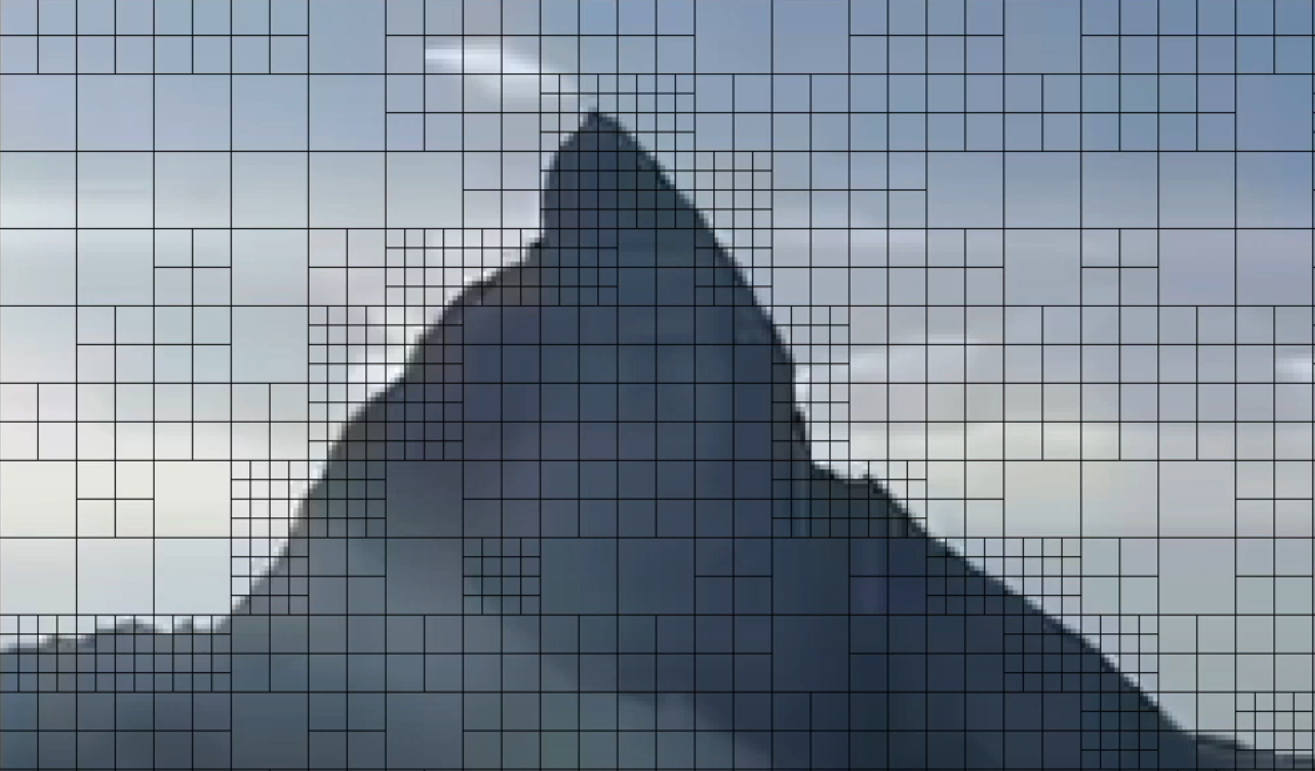
\includegraphics[width=1\textwidth]{images/macroblocks_sub-division.png}
    \caption{Suddivisione di un'immagine in macroblocks e prediction-blocks.}
    \label{fig:macroblocks_sub_division}
\end{figure}

\subsubsection{Intraframe/intra prediction}
\begin{figure}[h]
    \centering
    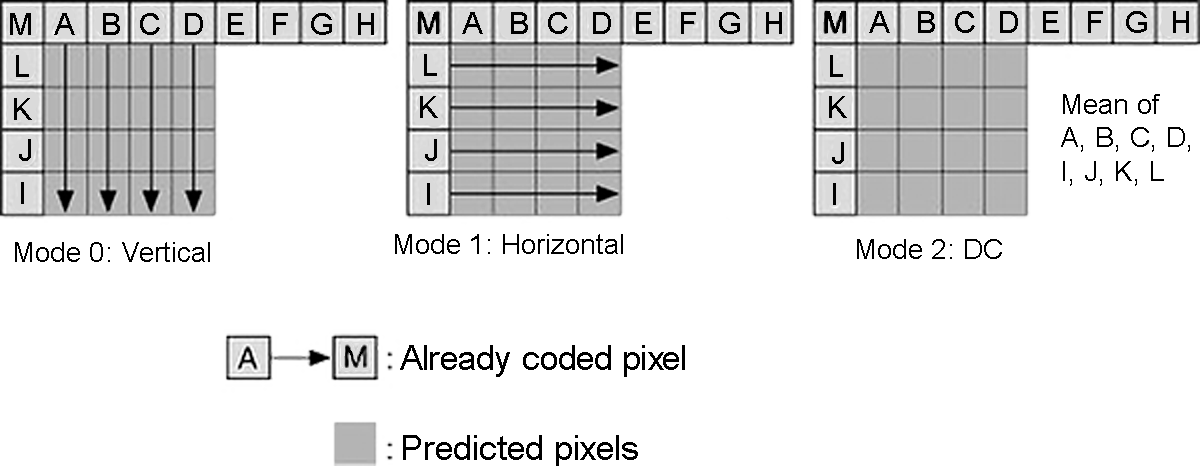
\includegraphics[width=1\textwidth]{images/intraframe-algo.png}
    \caption{Rappresentazione dei 3 metodi più utilizzati per la predizione intraframe}
    \label{fig:intraframe_algo}
\end{figure}

\noindent La compressione intraframe si riferisce alla compressione dei dati all'interno di
un singolo fotogramma. Questo metodo si divide in più passaggi:
\begin{enumerate}
  \item Per ogni macroblock o prediction-block, viene utilizzato un modello di predizione per stimare
  i valori delle matrici al suo interno basandosi sui valori delle celle adiacenti. Questo modello di
  predizione può essere semplice (es. facendo la media dei pixel adiacenti) o più complesso (come la
  predizione basata su modelli statistici o algoritmi di machine learning). Esistono in totale 9 metodi
  di previsione, ma i 3 metodi più frequenti sono (Vedi Figura~\ref{fig:intraframe_algo}) : traslando
  i pixel adiacenti già noti in orizzontale o in verticale, oppure facendo una media dei pixel adiacenti. Nel
  caso del formato H.264 ci sono in totale 9 algoritmi di intraframe.
  \item Successivamente, viene calcolata la residua, ovvero la differenza tra i pixel predetti e i
  pixel dell'immagine non compressa
  \item Infine, viene scelta la matrice residua, che si è avvicinata di più al gruppo di pixel originale,
  comprimendo così la dimensione del frame.
\end{enumerate}
È poi nella fase di intraframe che viene fatta la suddivisione dei macroblock in prediction-block.
L'algoritmo sceglie la suddivisione migliore provando tutti i tipi di divisioni dei
blocchi fino a trovare quello con la residua migliore.

\subsubsection{Interframe/Motion compensation}
Quando si parla di compressione, l'obiettivo è ridurre al minimo le ridondanze. Nel contesto dei video,
si nota subito che frame adiacenti temporalmente condividono una considerevole quantità di pixel.
L'algoritmo di interframe si occupa proprio di questo aspetto. Invece di analizzare i singoli frame uno
dopo l'altro, prende in considerazione più frame contemporaneamente per individuare le similitudini tra
di essi. Naturalmente, ci sono situazioni in cui ciò non è fattibile, come durante un cambio di scena,
dove la maggior parte o addirittura tutti i pixel possono cambiare da un frame all'altro.

Per prima cosa, qualora debba essere classificato ogni frame di un video, quest'ultimo viene
ridimensionato ad una risoluzione inferiore e per ogni frame si applicano sia l'algoritmo di intraframe,
che di interframe, e si comparano i due risultati. Se il costo\footnote{con costo si intende il peso
in termini di memoria calcolato attraverso un processo di comparazione tra i due metodi intraframe e interframe}
dell'intraframe è inferiore, questo
significa che il frame che si sta analizzando non ha elementi in comune con i frame precedenti,
suggerendo così un cambio di scena. Ci sono in totale 3 tipi di frame (vedi Figura~\ref{fig:frame_type}):

\begin{itemize}
  \item Il tipo \textbf{I frame} di solito indica un cambio di scena, pertanto si applica l'algoritmo
  di intraframe, poiché non ci sono altri frame di riferimento. Di conseguenza, questo è il frame meno
  compresso. 
  \item Il tipo \textbf{P frame} contiene solo la parte dell'immagine che è cambiata rispetto al fotogramma
  precedente o successivo, quindi si può applicare esclusivamente l'algoritmo di Interframe. Questo tipo di
  frame occupa circa il 50\% in meno di spazio rispetto al tipo I.
  \item Il tipo \textbf{B frame} è un ibrido tra i due precedenti, in quanto il frame corrente è un misto
  tra frame precedenti e successivi, ma che contiene elementi nuovi. Questo è il tipo di frame più
  efficiente in quanto occupa il 25\% dello spazio rispetto al tipo I.
\end{itemize}

\begin{figure}[h]
    \centering
    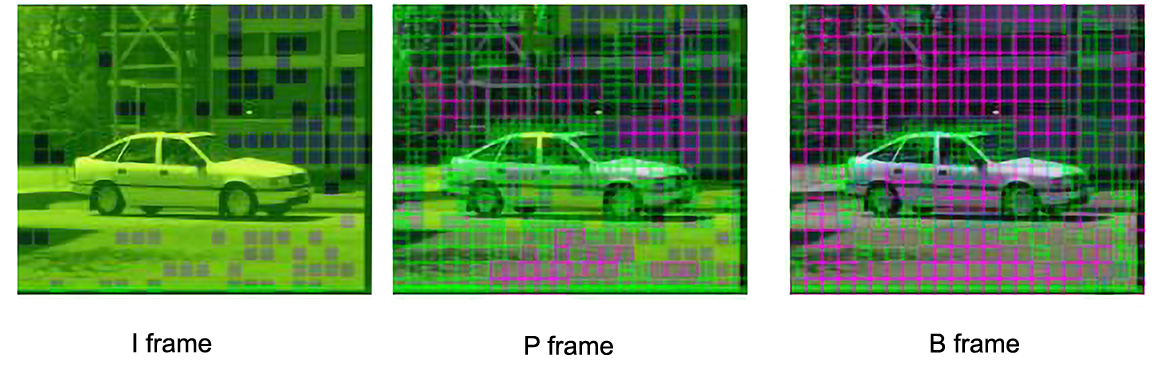
\includegraphics[width=1\textwidth]{images/frame-type.png}
    \caption{Classificazione del tipo di frame.
    I macroblock viola indicano che quel frame è stato ricostruito da un frame precedente,
    mentre quello verde che è stato codificato grazie ai pixel interni al frame.}
    \label{fig:frame_type}
\end{figure}

Nel dettaglio, per comprendere quali elementi di un frame vengono ripetuti all'interno di altri frame,
vengono nuovamente sfruttati i macroblock. Inoltre, i frame non vengono codificati in ordine cronologico,
ma in modo sparso, in modo che quando si analizza un frame che utilizza l'algoritmo di interframe, possa
attingere informazioni sia dai frame precedenti che da quelli successivi, come mostrato nella
Figura~\ref{fig:interframe}. Ci sono due modi per popolare un macroblock grazie al intraframe:

\begin{itemize}
  \item La \textbf{Uni-directional Motion Compensation} consiste nell'individuare il macroblock identico
  tra i frame precedenti o successivi e salvandolo come un \textbf{motion vector}, ovvero un vettore che
  identifica lo spostamento del macroblock tra i due frame.
  \item La \textbf{Bi-directional Motion Compensation} implica invece l'individuazione di due macroblock,
  uno nel frame successivo e uno in quello precedente, che più si avvicinano a quello in esame.
  Successivamente, si salvano i loro due motion vector e si combinano utilizzando una funzione matematica.
  Ad esempio, il codec H.264 calcola la media tra le due matrici, sottrae i pixel originali generando una
  matrice "residuo" e viene anch'essa memorizzata. Questo permette non solo di di memorizzare i
  macroblocks identici tra frame, ma anche di poter tracciare quelli che vengono ruotati, stirati o inclinati.
\end{itemize}

\begin{figure}[h]
    \centering
    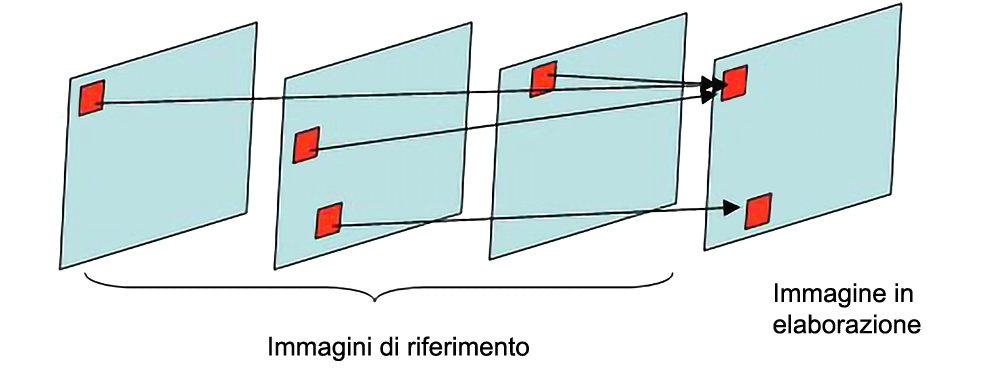
\includegraphics[width=1\textwidth]{images/interframe.png}
    \caption{Nella figura viene mostrato un esempio di come l'algoritmo di interframe
    attinge a frame diversi per ricostruire il macroblock interessato.}
    \label{fig:interframe}
\end{figure}

\subsubsection{Transformation}
Ora che tutti i macroblocks sono stati codificati secondo il metodo più conveniente, si prendono solo quelli che contengono
la matrice dei residui, ovvero quelli codificati mediante interframe, e vengono divisi in blocchi quadrati 8x8
e viene applicata la trasformata discreta del coseno (\textbf{DCT} - Discrete Cosine Transform).

La trasformata discreta del coseno permette di rilevare variazioni di informazioni (come il colore per
i blocchi Chroma o la luminosità per i blocchi Luma) trasformando i valori dei pixel dal dominio
spaziale al dominio delle frequenze e individuando così i blocchi con più dettagli, ovvero i blocchi
con frequenza maggiore.

Per applicare la trasformata discreta del coseno bisogna:

\begin{figure}[h]
    \centering
    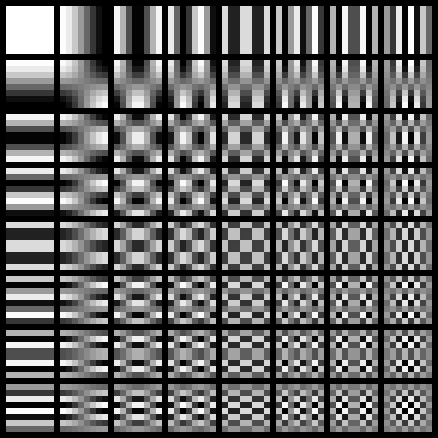
\includegraphics[width=0.8\textwidth]{images/DCT-table.png}
    \caption{Tabella DCT. In particolare si noti come partendo dall'angolo in alto a sinistra,
    più si va verso destra e più la frequenza della matrice aumenta in orizzontale e più si va
    verso il basso e più la frequenza della matrice aumenta in verticale.}
    \label{fig:DCT_table}
\end{figure}

\begin{enumerate}
    \item Dividere l'immagine (ovvero le 3 matrici dei residui) in piccoli blocchi quadrati 8x8
    \item Normalizzare i valori delle matrici sottraendo a ciascun valore 128; così facendo
    ogni cella sarà compresa tra 128 e -127. Se prendiamo ad esempio la matrice Lumen il valore
    128 corrisponderà al bianco, mentre il valore -127 al nero e i valori centrali saranno tutte
    le tonalità di grigio
    \item Successivamente, ricostruire la matrice 8x8 ottenuta come somma di matrici
    prese da una matrice DCT precalcolata (vedi figura Figura~\ref{fig:DCT_table}. Nella 
    Figura~\ref{fig:DCT_example} si può notare come partendo da un'immagine, si possa
    risalire ad essa mediante una somma di matrici prese dalla tabella DCT.
\end{enumerate}

\begin{figure}[h]
    \centering
    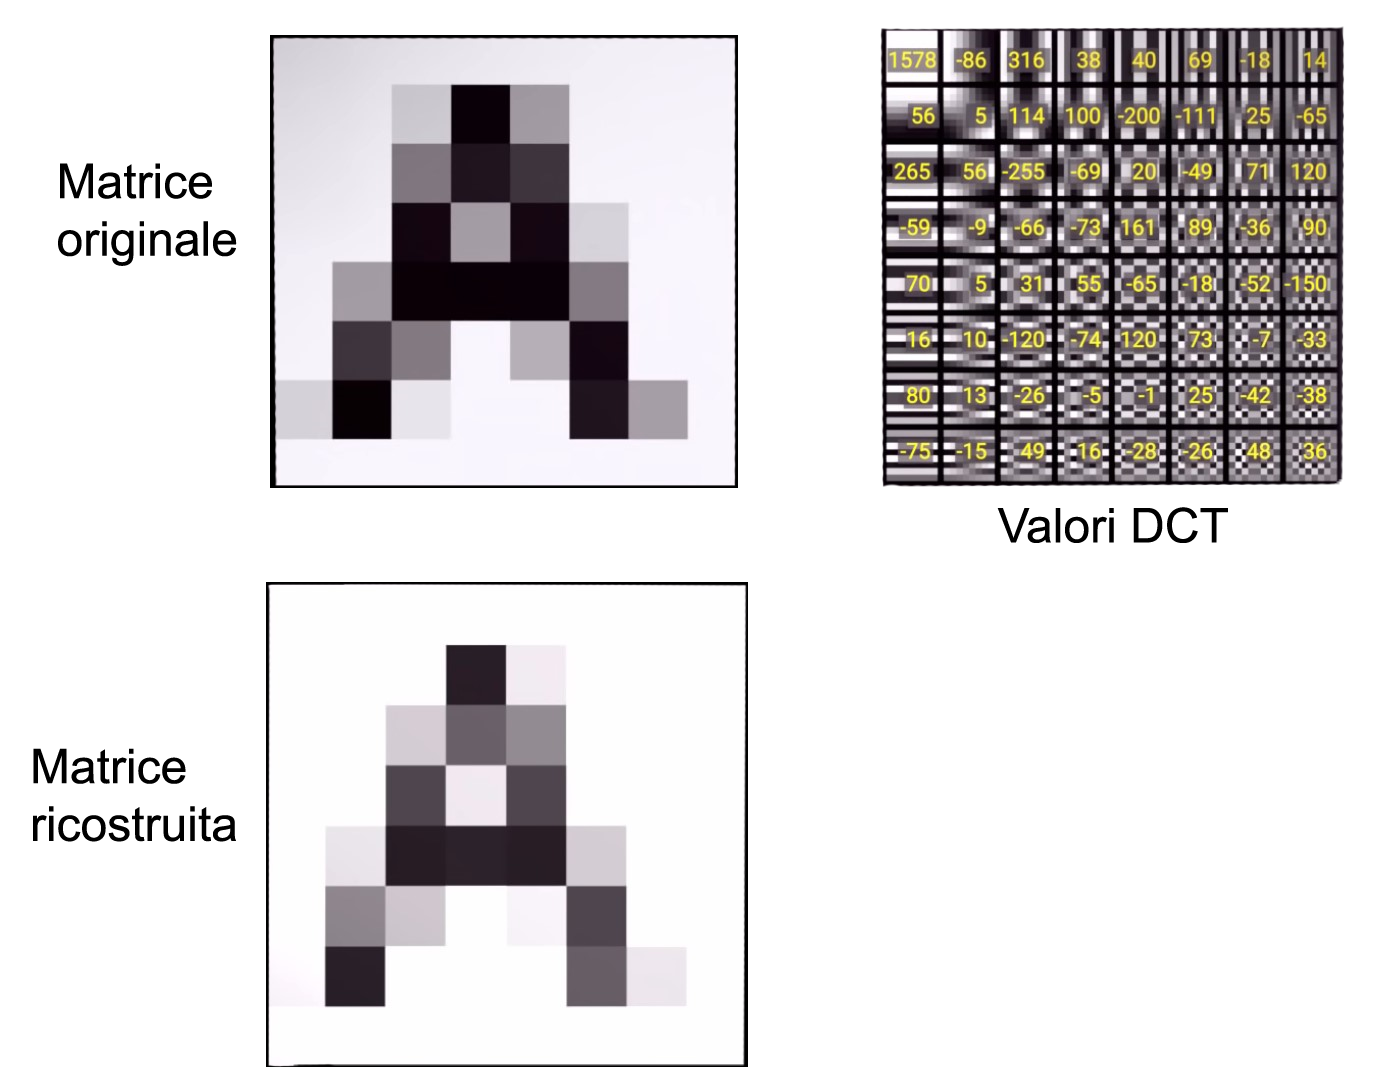
\includegraphics[width=1\textwidth]{images/DCT-example.png}
    \caption{Esempio di come una matrice (in alto a sinistra) mediante somma di matrici DCT
    più essere ricostruita.}
    \label{fig:DCT_example}
\end{figure}

\subsubsection{Quantization}
La quantizzazione implica la creazione di tre matrici, chiamate tabelle di quantizzazione, per
suddividere i valori delle matrici ottenute tramite la trasformazione. Queste tre matrici, una
per le Luma e due per le Chroma, sono identiche per l'intera immagine e sono strutturate in
modo che i valori più elevati si trovino nella parte inferiore destra, corrispondente alle
frequenze più alte nell'immagine DCT. Questo schema favorisce una migliore compressione nelle
aree in cui le frequenze dell'immagine sono più elevate.

Per quantizzare un blocco, ogni valore DCT viene diviso per il valore corrispondente nella
tabella di quantizzazione e successivamente arrotondato al numero intero più vicino (vedi
l'esempio della Figura~\ref{fig:quantization_example}). Questo processo riduce leggermente la
qualità dell'immagine, ma lo fa in modo intelligente, rimuovendo dettagli dalle aree ad alta
frequenza, impercettibili per l'occhio umano.

\begin{figure}[h]
    \centering
    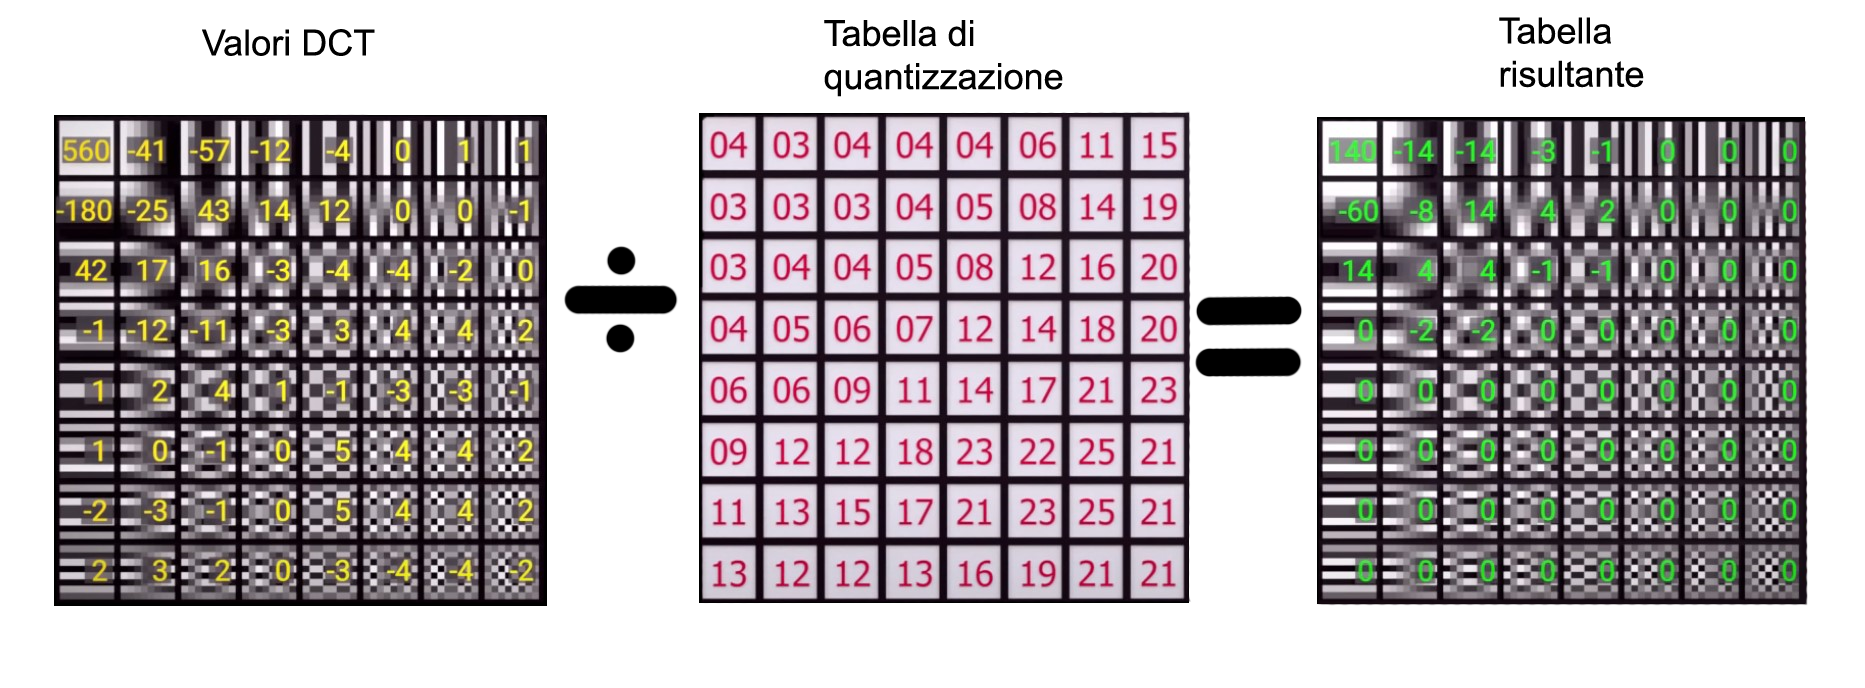
\includegraphics[width=1\textwidth]{images/quantization-example.png}
    \caption{Esempio di quantizzazione della matrice DCT.}
    \label{fig:quantization_example}
\end{figure}

\subsubsection{Entropy Coding}
Nella fase di Entropy Coding, si mira a comprimere ulteriormente i dati, facendo riferimento non
all'immagine come tale, ma interpretandola come una stringa di bit o simboli. Esistono diversi tipi di
algoritmi di Entropy Coding che possono variare in base al codec e all'implementazione.
Tra i più importanti vi è l'\textbf{Arithmetic codec}, il quale cerca di predire i prossimi
simboli o bit in base a una serie data di simboli e a una tabella di probabilità. Durante ogni fase
della codifica di un video, viene applicato un algoritmo di codifica diverso o leggermente
modificato. Un altro algoritmo di codifica degno di nota è la \textbf{codifica di Huffman}, o
Huffman encoding, rinomato per la sua flessibilità. Oltre ad essere utilizzato nella codifica video,
trova infatti impiego anche nella codifica delle immagini (come nella JPEG), nella codifica audio
(come nella MP3) e nella compressione dei file (come nei formati PKZIP, ZIP e WinRar).

Nella codifica video, la \textbf{codifica di Huffman} subisce leggere modifiche e viene impiegata
in combinazione con l'algoritmo \textbf{Run Length}. Quest'ultimo viene applicato alle matrici
quantizzate, come discusso nel paragrafo precedente. In questo contesto, i valori delle matrici vengono
letti "a zig-zag", partendo dall'angolo in alto a sinistra e procedendo verso il basso a destra.
Questo schema di lettura organizza i valori in modo tale che quelli con frequenza più alta, spesso 
rappresentati da sequenze di zeri consecutive, si trovino verso la fine della sequenza. Una volta ottenuta
la lista di numeri, quando si incontrano due o più numeri ripetuti si tiene conto di quante volte un certo
numero si è ripetuto invece di riscrivere ogni volta lo stesso numero (vedi l'esempio della
Figura~\ref{fig:huffman_example})).

\begin{figure}[h]
    \centering
    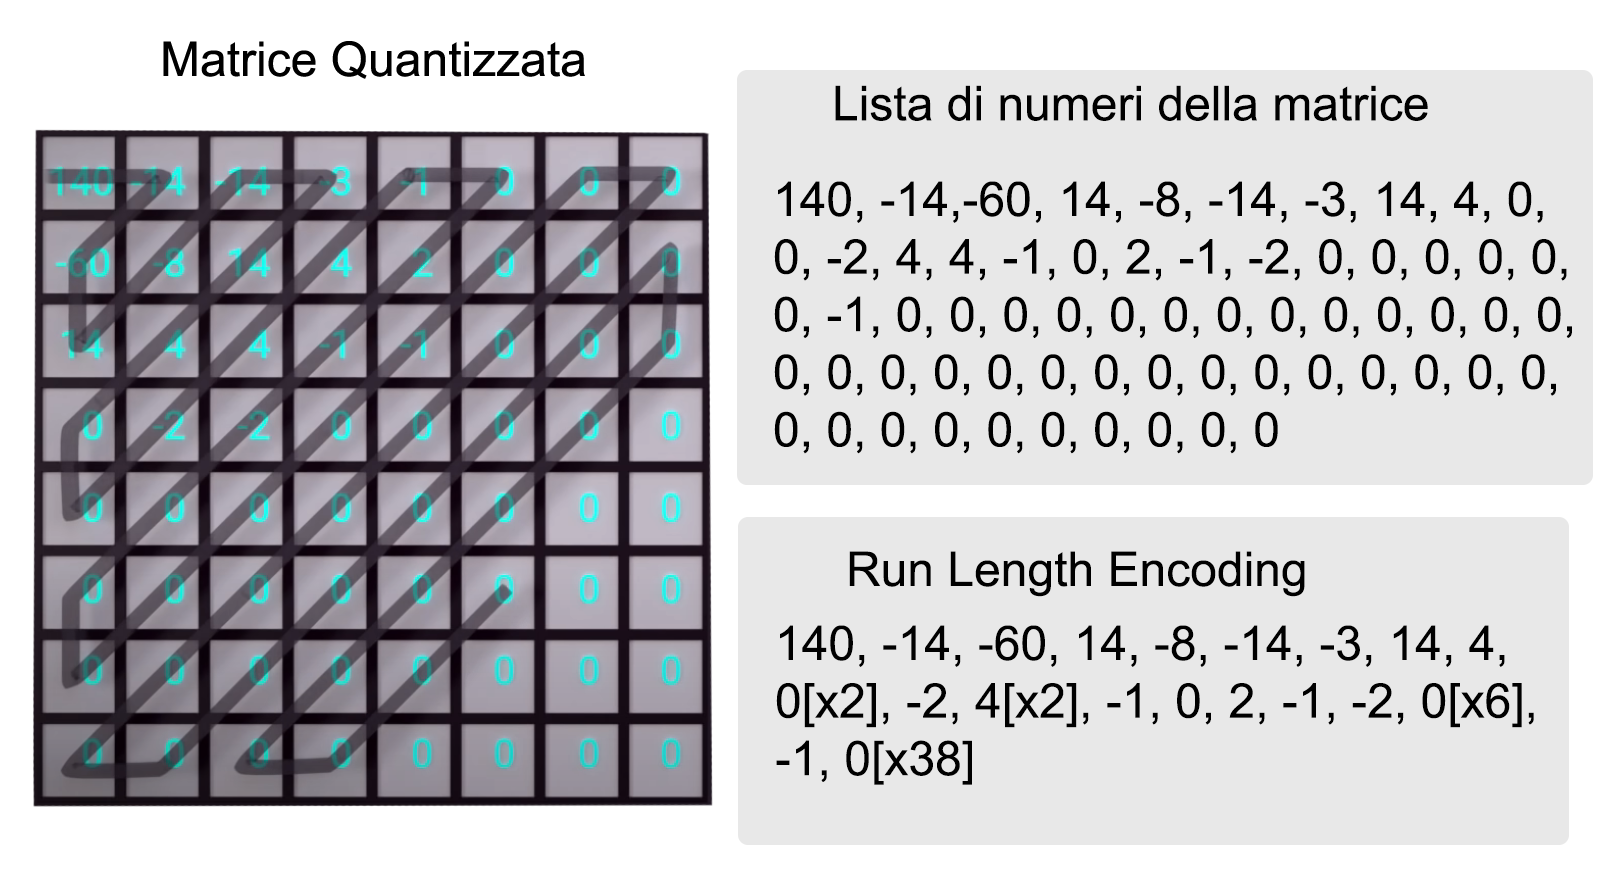
\includegraphics[width=1\textwidth]{images/huffman-example.png}
    \caption{Esempio della codifica di Huffman e Run Length.}
    \label{fig:huffman_example}
\end{figure}

Una volta ottenuta una lista con tutti i numeri e la loro frequenza, possiamo procedere applicando
la \textbf{codifica di Huffman} \footnote{Nota come in questo paragrafo verrà spiegato come l'algoritmo
viene applicato alla codifica video, se interessati ad una visione più ampia,
\href{https://www.youtube.com/watch?v=JsTptu56GM8}{questo video} lo spiega nel dettaglio con tanto
di illustrazioni}. L'algoritmo è diviso in diversi passaggi:

\begin{enumerate}
    \item Si ordina la lista precedentemente ottenuta in base alla frequenza dei simboli.
    \item Si prendono gli ultimi due elementi e si inizia a costruire un piccolo albero con alla base i due
    elementi selezionati e come "padre" la somma di tutti i "figli".
    \item Si prende l'oggetto albero appena creato e lo si reinserisce nella lista nella posizione dettata
    della sua frequenza.
    \item Si procede in questo modo fino a quando la lista sarà composta da un solo elemento.
\end{enumerate}

\begin{figure}[h]
    \centering
    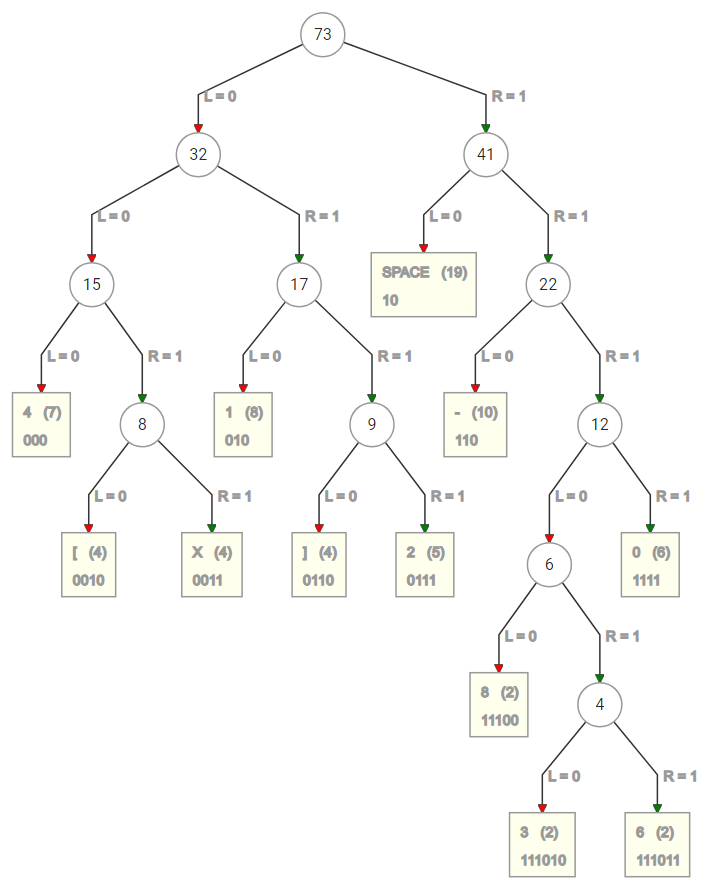
\includegraphics[width=0.75\textwidth]{images/huffman-tree.png}
    \caption{Esempio di un albero di Huffman costruito con i valori ottenuti grazie all'algoritmo
    Run Length.}
    \label{fig:huffman_tree}
\end{figure}

A questo punto, si dispone di un vasto albero che contiene tutti i numeri della lista insieme alle
rispettive frequenze (consultare la Figura~\ref{fig:huffman_tree}). Ora, per codificare ciascun numero,
che ricordiamo variare da -127 a 128, non è più necessario utilizzare 8 bit, ma in molti casi molto
meno. Abbiamo trasformato il processo di codifica da una rappresentazione binaria diretta di ciascun
numero a un'indicazione degli indici dell'albero, dove ogni sequenza di 0 e 1 determina la direzione
da seguire nell'albero per raggiungere il simbolo desiderato.

Prendendo in considerazione l'esempio illustrato nella Figura~\ref{fig:huffman_example}, inizialmente
la matrice occupava uno spazio di 8x8x8, equivalenti a 512 bit. Dopo l'applicazione degli algoritmi
Run Length e Huffman, il consumo di spazio si riduce drasticamente a soli 239 bit, permettendo un
risparmio di circa il 46\% dello spazio. L'esempio riportato non è ottimale in quanto alcuni simboli
sono superflui (come lo spazio e le due parentesi quadre), ma sono stati lasciati per rendere
l'esempio più esplicativo. Consultando l'albero si può notare come il passaggio di normalizzazione
dei valori, ovvero sottrarre 128, abbia incrementato la compressione dei dati, in quanto ha aumentato
la probabilità di avere due numeri identici. Per esempio i numeri 98 e 158 avrebbero richiesto due
rami differenti all'interno dell'albero di Huffman, ma grazie alla normalizzazione si avranno -30 e
30, che occuperanno solo un ramo in quanto il simbolo '-' sarà quasi sicuramente utilizzato per altri
numeri.

\subsubsection{Loop filtering}
Il \textbf{Loop filtering} è una tecnica che viene utilizzata solo nella ricostruzione delle immagini,
non nella codifica, e consiste nell'applicare un o più filtri all'immagine apportando i seguenti benefici:

\begin{itemize}
    \item \textbf{Deblocking filter}: L'artefatto di blocco è un effetto causato dalla divisione del frame
    in blocchi più piccoli durante la compressione, creando delle linee di separazione tra di esse.
    Per questo problema viene utilizzato il deblocking filter, che aiuta a ridurre l'effetto di questo
    artefatto, migliorando l'aspetto generale del video (vedi Figura~\ref{fig:deblocking_filter}). La
    tecnica consiste nell'applicare tanti piccoli filtri 4x4 lungo i bordi dei blocchi.
    Questo è il filtro più importante in quanto è presente in quasi tutti i formati di compressione video.
    \item \textbf{Riduzione del rumore}: Il rumore video può manifestarsi durante la compressione
    o a causa delle condizioni di trasmissione. Il loop filtering può ridurre questo rumore,
    migliorando la chiarezza complessiva dell'immagine.
    \item \textbf{Smoothing dei contorni}: Per migliorare la qualità visiva, il loop filtering può
    applicare un effetto di smoothing ai contorni dell'oggetto, rendendo l'immagine più gradevole e
    meno soggetta a artefatti visivi.
    \item \textbf{Miglioramento della compressione}: Una filtrazione efficace può ridurre la quantità
    di dati richiesti per rappresentare un video, migliorando quindi l'efficienza della compressione
    senza compromettere eccessivamente la qualità visiva.
\end{itemize}

\begin{figure}[h]
    \centering
    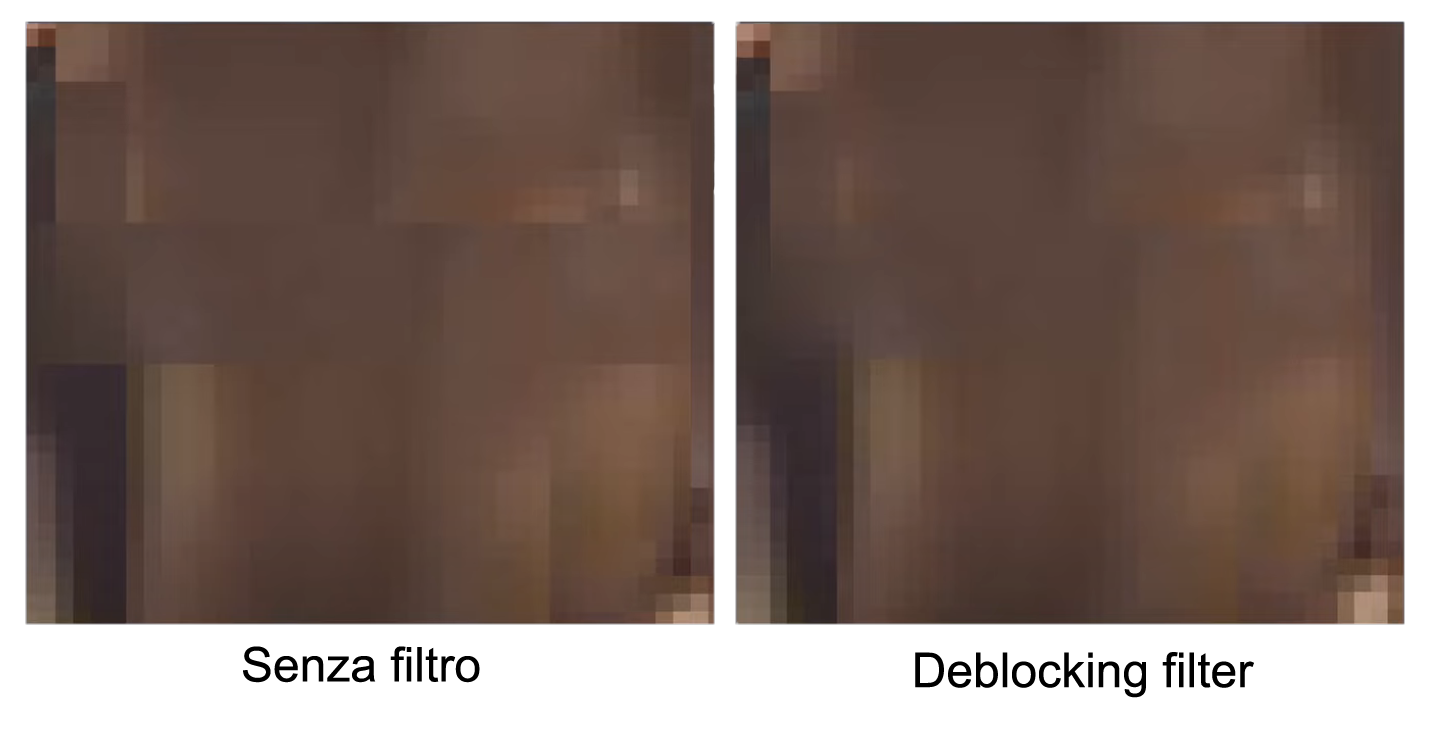
\includegraphics[width=1\textwidth]{images/deblocking-filter.png}
    \caption{Esempio di come il deblocking filter riduce gli artefatti tra i blocchi. Nell'immagine di
    sinistra si può chiaramente vedere la linea di separazione tra i due blocchi.}
    \label{fig:deblocking_filter}
\end{figure}

\subsubsection{Ricapitolando}
\begin{figure}[h]
    \centering
    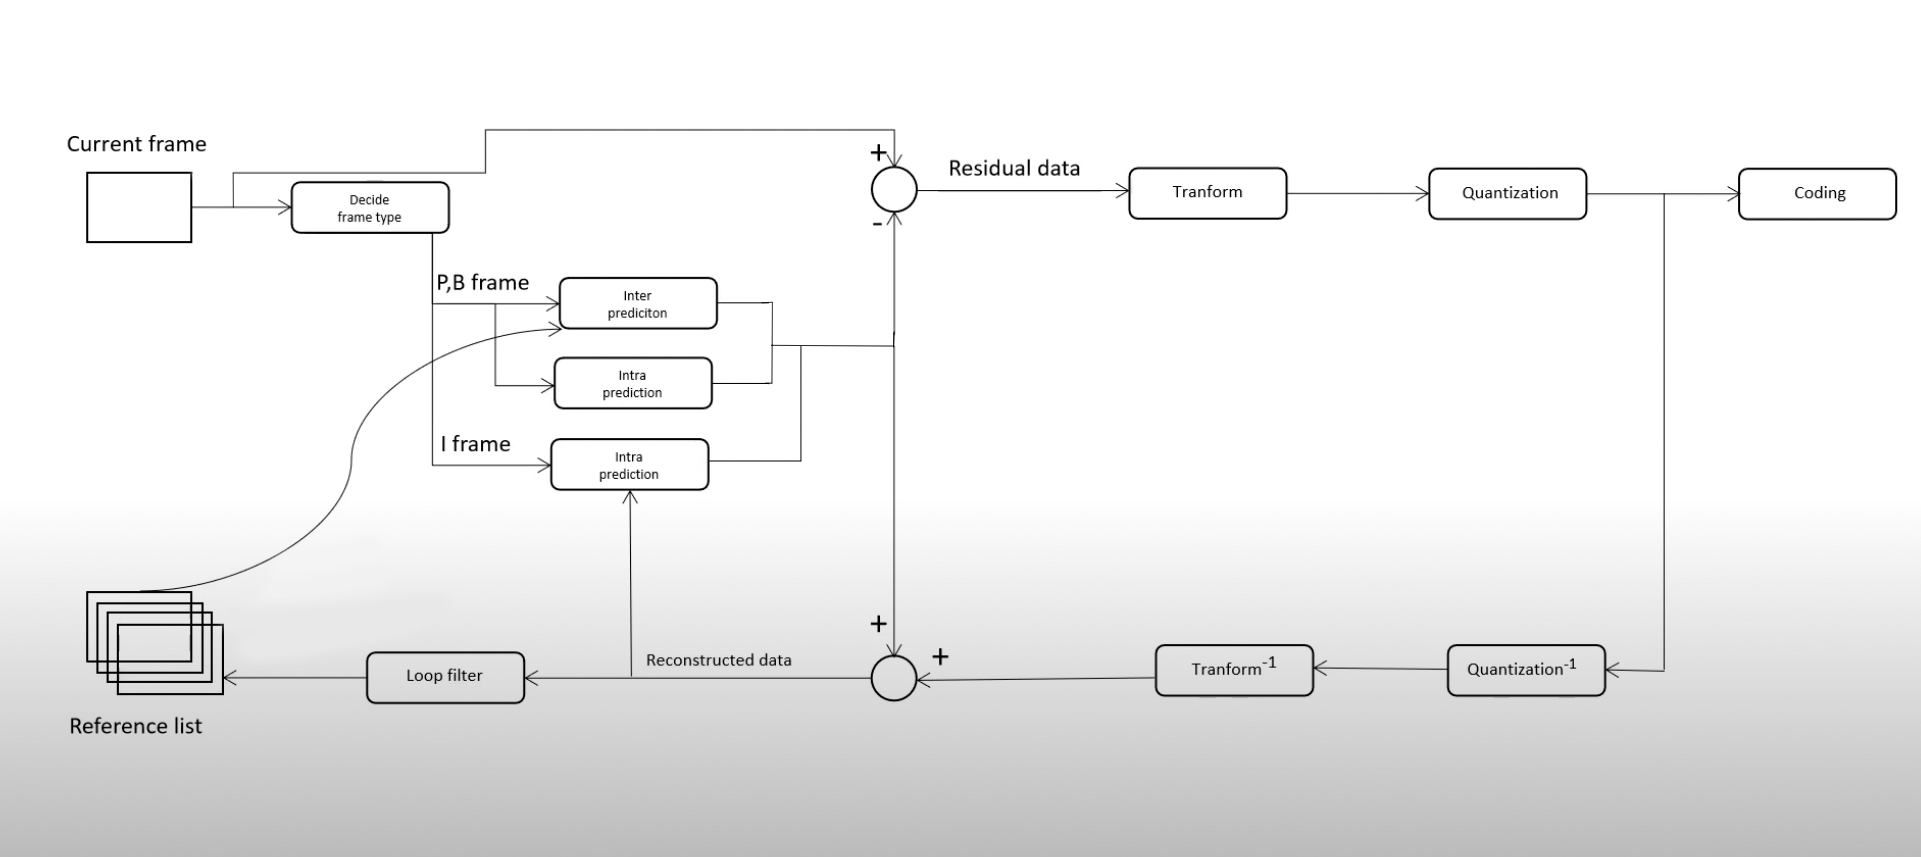
\includegraphics[width=1\textwidth]{images/h264-coding-loop.png}
    \caption{Ciclo di codifica di un frame all'interno del formato H.264.}
    \label{fig:h264_coding_loop}
\end{figure}

\noindent Per riassumere, il processo di compressione inizia con la lettura del file video e la
suddivisione in frame. Ogni frame subisce una conversione dal formato RGB a YCrCb, e viene
selezionato il tipo di frame. Successivamente, vengono applicati algoritmi di intra e inter prediction
ai macroblocks dei residui, seguiti dalla trasformazione e quantizzazione. Infine, si utilizza la
codifica di entropia per comprimere l'immagine a livello di bit, seguita dall'applicazione di vari
filtri per migliorare la naturalezza dell'immagine.

Come abbiamo visto, la compressione e soprattutto la decodifica in tempo reale di un video richiedono
considerevole potenza di calcolo. Il formato H.264 è stato uno dei primi codec a necessitare di un
acceleratore hardware dedicato per la decodifica dei video, poiché le operazioni computazionali richieste
diventavano sempre più complesse. Questo portò alla luce che con l'avanzare delle nuove tecnologie per
la compressione dei video, che riducevano le dimensioni dei file, aumentava anche la potenza di calcolo
necessaria per la codifica e decodifica dei video.

---
TODO: parte da rivedere e da posizionare meglio
Le differenze principali con il codec H.261 sono

- supporto di più dimensioni per la chroma subsampling
- slice di dimensioni variabili, quanto nel vecchio codec ogni slice aveva una dimensione prefissata
- supporto a DVD, ATV, HDTV
- i motion vector non sono più limitati a spostare i macroblocks all'interno della loro griglia
(ovvero che un macroblock deve per forza stare al posto di un altro), ma possono anche indicare una
posizione con una precisione di 1/4 di macroblock.
- predizione dei movimenti  (da controllare)
- la trasformazione discreta del coseno (DCT)
- la compensazione del movimento (da controllare)

Introduce la possibilità di codificare fino a 4k, poi più avanti arriva fino all'8k.
Youtube lo ha usato fino al 2010 per poi abbandonarlo in favore del proprio VP8.
---

\subsection{H.265/HEVC}
Con l'avanzare delle tecnologie e dell'informatizzazione di un pubblico sempre più vasto
è nato il problema di come rappresentare i nuovi formati video e di come poter comprimere ulteriormente
questi file. Per questo motivo nel 2013 la \textbf{International Telecommunication Unit} ha creato il
nuovo codec H.265, che non solo è in grado di comprimere meglio i filmati (considerando che il 4k sta
prendendo sempre più piede in questo periodo) ottenendo una compressione migliore del 50\% rispetto all'H264, ma
riesce a codificare filmati 3D, in HDR e anche video girati in 360°. Nei paragrafi successivi si vedremo quali
cambiamenti sono stati apportati al predecessore H.264 per creare questo nuovo codec.

\subsubsection{Coding Tree Unit (CTU)}
La prima differenza con il formato H.264 è la gestione dei blocchi. Il codec H.265 non utilizza
i classici macroblocks che sono stati usati fino a questo periodo dalla maggioranza dei codec, ma
utilizza il sistema \textbf{Coding Tree Unit} (d'ora in poi verrà abbreviato con CTU). A differenza
dei macroblocks che sono di dimensione variabili 16x16, i CTU hanno tutte dimensioni identiche
64x64, 32x32 o 16x16 all'interno di un frame (questo parametro dipende dal bitrate selezionato all'inizio
della codifica,inoltre CTU di dimensioni più grandi permettono una codifica più efficiente e una resa
grafica più alta, a discapito del tempo di codifica, che cresce esponenzialmente). Le CTU, come i
macroblocks, sono divisi nei tre sotto blocchi, uno per la Luma e 2 per le Chroma, chiamati \textbf{Coding Tree Block} o CTU.
Un grosso problema delle CTU è che sono troppo grandi per poter eseguire gli algoritmi di inter e intra
prediction e per ciò ogni CTU viene ulteriormente divisa in \textbf{Coding Block} (CB), che possono avere
dimensioni variabili da 32x32 fino a 8x8.
Le Coding Block sono le unità più piccole su cui lavorare e si possono distinguere in due tipi:

\begin{itemize}
    \item \textbf{Prediction Block} (PB) se si sta usando un algoritmo di Interframe. Questi sono
    gli unici tipi di blocchi che possono essere suddivisi in 2, creando dei rettangoli.
    \item \textbf{Transform Block} (TB) se si sta usando un algoritmo di Intraframe, quindi contiene
    dati sulle residue delle immagini.
\end{itemize}

Come detto precedentemente, le CTU sono divise in 3 CTB per ogni matrice di Luma/Chroma; la stessa
cosa vale per le componenti sottostanti, quindi esiste una \textbf{Prediction Unit} (PU) che contiene
a sua volta tre Prediction Block e così via. Non solo gli oggetti "Unit" oltre ai blocchi di matrici
contengono un relativo \textbf{Syntax Element} che tiene traccia di come un determinato blocco è
stato codificato, ad esempio la Syntax Element di una Coding Unit contiene le informazioni circa
 il tipo di algoritmo (Intraframe o Interframe) che è stato utilizzato (vedi Figura~\ref{fig:coding_unit}).
 
 \begin{figure}[h]
    \centering
    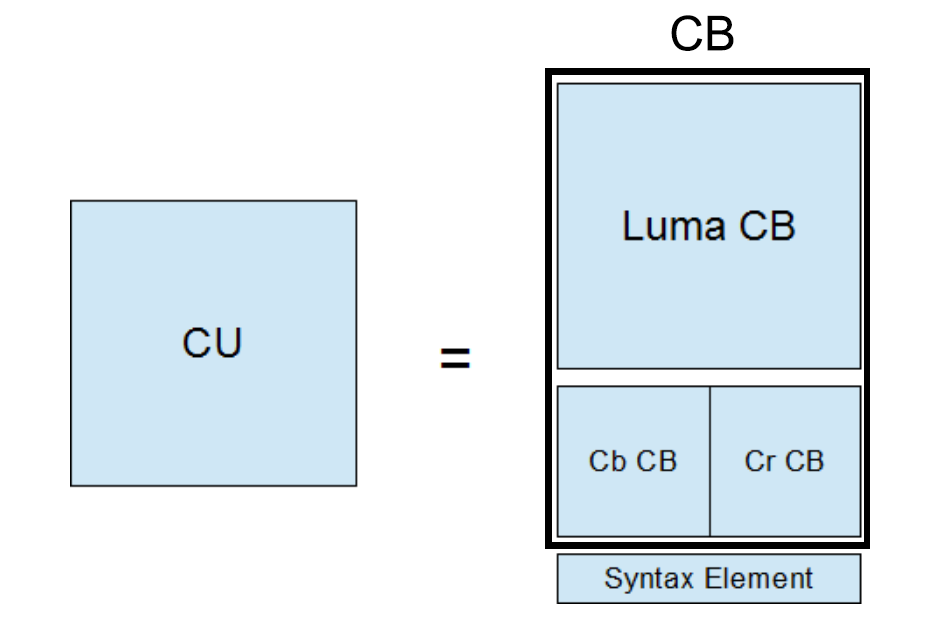
\includegraphics[width=0.8\textwidth]{images/coding-unit.png}
    \caption{Rappresentazione di come viene suddivisa una Coding Unit.}
    \label{fig:coding_unit}
\end{figure}

 \noindent Ogni CTB è suddiviso al suo interno come un albero che memorizza le informazioni mediante un algoritmo
chiamato Z-Scan, rappresentando un pattern "a zig-zag" (come si può intuire dalla
Figura~\ref{fig:chroma_CTB}).
Una caratteristica che i CTU hanno in comune con i macroblocks è la gestione dei "blocchi",
in quanto anche i CTU vengono gestiti e processati in gruppi chiamati \textbf{slice}.

\begin{figure}[h]
    \centering
    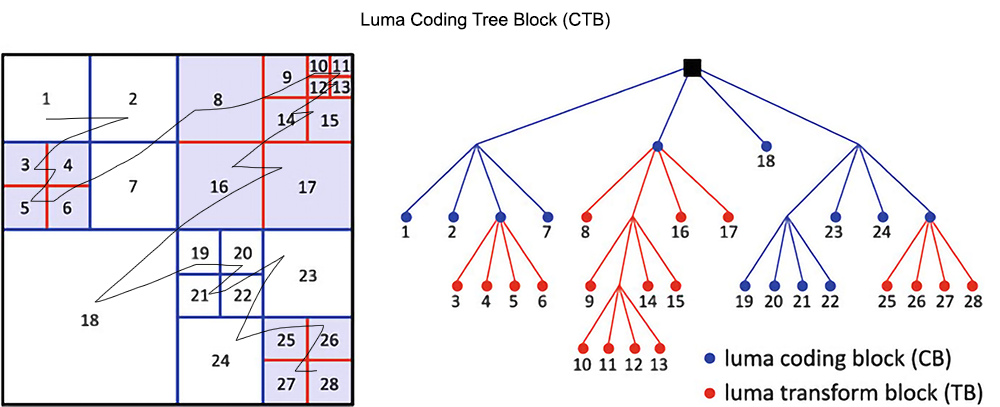
\includegraphics[width=0.8\textwidth]{images/chroma-CTB.png}
    \caption{Rappresentazione di una Luma CTB e di come i sotto blocchi vengono letti e inseriti
    all'interno dell'albero.}
    \label{fig:chroma_CTB}
\end{figure}

Una dettaglio molto importante è che all'interno di un Coding Block, ogni Prediction Block utilizza la
stessa modalità di predizione (intra o inter).

\subsubsection{Intraframe/intra prediction}
A cambiare nell'applicazione della intra prediction sono i blocchi, che possono avere molte più
dimensioni rispetto all'H.264, con lati da 8, 16, 32, 64 e tutte le combinazioni di quadrati o rettangoli
possibili, garantendo una compressione migliore.

Inoltre, le modalità di previsione non sono più solo 9, che all'epoca della risoluzione più diffusa di 720p
erano più che sufficienti, ma ben 35. Tra queste, vi sono una modalità di previsione planare, una previsione DC 
e 33 previsioni angolari (vedi Figura~\ref{fig:HEVC_intra}).

\begin{figure}[h]
    \centering
    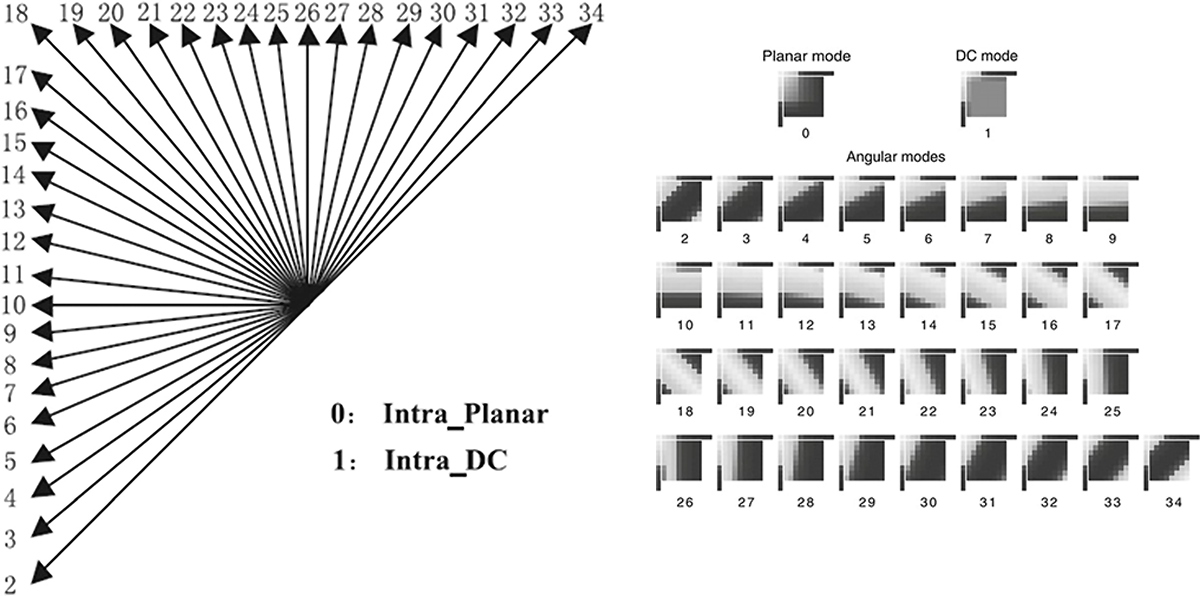
\includegraphics[width=0.8\textwidth]{images/HEVC-intra.png}
    \caption{A sinistra, una rappresentazione di tutte le direzioni in cui si può applicare la Intraframe,
    mentre a destra un esempio di come ciascun algoritmo viene applicato su ciascun blocco.}
    \label{fig:HEVC_intra}
\end{figure}

TODO: spiegare matematicamente come vengono applicate queste due nuove modalità (vedi video ~ 13:20). Lo devo fare?

Inoltre, dopo la ricostruzione di un blocco, viene applicato un filtro di smoothing per rendere
l'immagine più gradevole. Questo viene fatto solo sui blocchi Luma in quanto hanno un impatto visivo più
importante dei Chroma perché si risparmia sulla potenza computazionale.
Infine, la DCT non è più limitata a una dimensione di 8x8, ma può arrivare anche a dimensioni di 32x32,
aumentando ulteriormente la compressione.

\subsubsection{Interframe/Motion compensation}
Anche il codec H.265 utilizza la Interframe, esattamente come il suo predecessore, ma i motion vector che
utilizza non sono più limitati a spostare un blocco sulla posizione esatta di un altro blocco di un frame,
ma possono traslare un Coding Block (CB) in qualsiasi posizione del frame desiderata.

Nella Interframe, vengono aggiunte altre tre tecnologie per aumentare la compressione:

\begin{itemize}
    \item \textbf{Merge Mode}: Questo metodo utilizza la correlazione spaziale e temporale per ridurre la
    ridondanza dei parametri di movimento tra i blocchi adiacenti. In poche parole, una Prediction Unit
    (PU) prende i parametri di movimento (motion vector) dalle PU adiacenti per massimizzare l'efficienza.
    Questo risultato può essere ottenuto copiando il motion vector di una PU vicina, oppure facendo una
    media di più PU vicine (si noti che con PU vicine non si intendono solo le PU adiacenti fisicamente, ma
    anche temporalmente).
    \item \textbf{Advanced Motion Vector Prediction} (AMVP): Simile al Merge Mode, ma invece di copiare i
    motion vector dalle PU adiacenti, l'AMVP li analizza tutti e fa una predizione su quale sarà il motion
    vector della PU in analisi. Se la predizione è sufficientemente precisa, utilizza il vettore predetto
    invece di memorizzarne uno nuovo.
    \item \textbf{Weighted Prediction}: In casi dove un video presenta una scena con un'animazione di fade
    (l'immagine diventa progressivamente più scura fino a diventare nera, per poi tornare lentamente alla
    luminosità naturale), il codec H.264 creerebbe due scene distinte con due I-frame. Al contrario, il
    nuovo codec H.265 riconosce questi pattern e genera una Weighted Prediction, creando un solo I-frame
    all'inizio della scena e, durante l'animazione di fade, riduce semplicemente l'intensità della matrice
    Luma.
\end{itemize}

\subsubsection{Transformation e Quantization}
Nella trasformazione, il codec H.265 introduce la tecnologia Residual Quad-tree Transform (RQT), utilizzata
all'interno delle TB, che possono avere dimensioni variabili. Questa innovazione consente l'applicazione di
trasformate diverse a blocchi di grandi dimensioni rispetto a quelli piccoli, permettendo così di mantenere
più dettagli nei blocchi più piccoli. Nei blocchi grandi, impiegati per rappresentare aree uniformi con
pochi dettagli, si ottiene un'elevata compressione a scapito di una qualità mediocre del dettaglio. Tale
deficit è accettabile poiché le suddette aree sono solitamente prive di dettagli significativi. La
regolazione del dettaglio avviene attraverso la creazione delle TB, che possono variare in dimensione
da 4x4 a 32x32, permettendo così di regolare il livello di dettaglio mantenuto in base all'area analizzata.
La tecnologia RQT prende il nome dal fatto che vengono utilizzate delle \textbf{Quadtree} per memorizzare
le TB, come illustrato dai rami rossi nella Figura~\ref{fig:chroma_CTB}.

Nella Quantizzazione, viene modificato anche il metodo della Discrete Cosine Transform (DCT), non viene
più utilizzata una scansione fissa predefinita per convertire i blocchi di pixel in coefficienti di frequenza, come accadeva in precedenza,
quando la tabella DCT veniva costruita cambiando i parametri verticali e orizzontali per un totale di 64 (8x8)
combinazioni.
L'Adaptive Scan Order (ACS) determina invece una sequenza di scansione ottimale per ciascun blocco di pixel,
considerando le caratteristiche spaziali e di frequenza del contenuto. ACS viene eseguita in sotto-blocchi
4×4 per tutte le dimensioni di blocco (TB), utilizzando una sola regione di coefficienti per la dimensione
del blocco 4×4 e più regioni di coefficienti 4×4 all'interno di blocchi di trasformazione più grandi. Vengono
selezionati tre metodi di scansione dei coefficienti: diagonale verso l'alto-destra, orizzontale e verticale
(vedi Figura~\ref{fig:HEVC_ACS}) implicitamente per la codifica dei coefficienti di trasformazione delle
dimensioni TB 4×4 e 8×8 nelle regioni predette all'interno dell'immagine. La selezione dell'ordine di
scansione dei coefficienti dipende dalle direzionalità della Intraframe. La scansione verticale viene
utilizzata quando la direzione di predizione è vicina all'orizzontale e la scansione orizzontale viene
utilizzata quando la direzione di predizione è vicina alla verticale. Per altre direzioni di predizione,
viene utilizzata la scansione diagonale verso l'alto-destra. Per i coefficienti di trasformazione nelle
modalità di predizione interframe di tutte le dimensioni di blocco e per i coefficienti di trasformazione
di predizione Interframe di 16×16 o 32×32, viene applicata esclusivamente la scansione diagonale verso
l'alto-destra 4×4 a sotto-blocchi di coefficienti di trasformazione.

\begin{figure}[h]
    \centering
    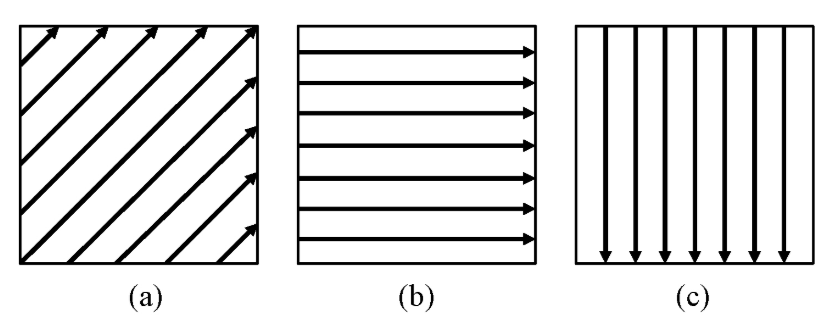
\includegraphics[width=0.8\textwidth]{images/HEVC-ACS.png}
    \caption{Rappresentazione dei tre approcci dell'algoritmo ACS.}
    \label{fig:HEVC_ACS}
\end{figure}

\subsubsection{Entropy Coding}
La Entropy Coding del codec H.265 è rimasta invariata rispetto al suo predecessore per quanto riguarda
la codifica delle matrici residue, continuando a utilizzare la codifica di Huffman. Tuttavia, è stato
introdotto un nuovo metodo per la codifica dei Syntax Element di ogni blocco e dei vettori di movimento.
Questo nuovo metodo è chiamato \textbf{Context Adaptive Binary Arithmetic Coding (CABAC)}, che si divide
in diverse fasi:

\begin{enumerate}
    \item \textbf{Binarization}: Il primo passo nella codifica CABAC è convertire i simboli
    non binari (come i coefficienti di trasformata o i valori di movimento) in una serie di simboli binari.
    Questa rappresentazione binaria è necessaria perché CABAC opera a livello di bit. Infine, questo enorme
    flusso di bit viene suddiviso in tanti piccoli flussi chiamati \textbf{Binary String}, che uniti formano
    il flusso originale.
    \item \textbf{Context Modeling}: In questa fase si crea una mappa dove ogni Binary String viene
    aggiunta ad una tabella che contiene la stringa stessa e il \textbf{Binary Index}, che non solo
    tiene traccia della posizione in cui si trova la Binary String, ma indica anche il numero di "1"
    presenti (vedi Figura~\ref{fig:CABAC_regular}). Il Context Modeling ha due modalità di esecuzione,
    quella appena descritta è la \textbf{regular mode}, mentre esiste anche la \textbf{bypass mode}
    che non comprime per nulla il flusso di bit, ma li codifica così come sono.
    
    \begin{figure}[h]
        \centering
        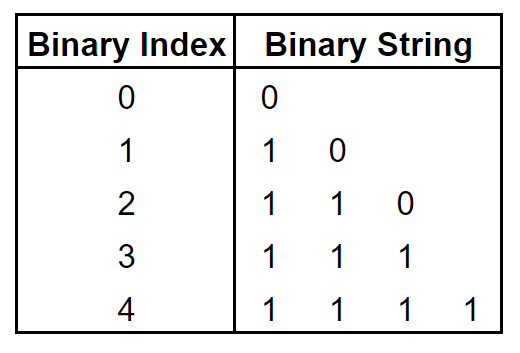
\includegraphics[width=0.5\textwidth]{images/CABAC-regular.png}
        \caption{Rappresentazione della fase di Context Modeling in regular mode della CABAC.}
        \label{fig:CABAC_regular}
    \end{figure}
    
    \item \textbf{Binary Arithmetic Codec (BAC)}: Il CABAC utilizza la codifica aritmetica, che è una forma
    avanzata di codifica di entropia senza perdita. Questa tecnica sfrutta la probabilità che un certo simbolo
    ("0" o "1") appaia, basandosi sul contesto fornito dalla sequenza di simboli precedenti. CABAC adatta
    dinamicamente il modello di probabilità in base ai simboli già codificati, migliorando così l'efficienza
    della compressione.
\end{enumerate}

\subsubsection{Loop filtering}
Come il codec H.264, anche questo applica molti filtri per migliorare la qualità dell'immagine, ma i principali
sono due, ovvero il \textbf{Deblocking Filter} e il \textbf{Sample Adaptive Offset (SAO)}.

L'algoritmo del Deblocking Filter rimane quasi invariato rispetto al predecessore, l'unico cambiamento che sussiste è che invece
di applicare un filtro 4x4 per ogni pixel lungo i bordi dei blocchi, applica dei filtri più grandi 8x8 più
leggeri affiancati uno all'altro. Questo viene fatto in quanto gli artefatti dovuti alla divisione in blocchi
sono meno evidenti, inoltre dato che i filtri sono affiancati e non sovrapposti, questo permette di calcolarli
in parallelo.

Per quanto riguarda la tecnica SAO, questo interviene dopo aver applicato la quantizzazione inversa durante
la decodifica. Analizza il contenuto dell'immagine e applica offset ai pixel in base ai valori dei pixel
circostanti. Con il termine offset si intende che ai valori delle matrici di Luma o Chroma vene aggiunto un
numero (ovvero l'offset).
In particolare:

\begin{enumerate}
    \item \textbf{Classificazione dei Pixel}: Il SAO divide i pixel dell'immagine in diverse categorie basate
    sulle loro caratteristiche locali. Queste categorie possono essere determinate in base al valore del pixel
    rispetto ai pixel vicini. In particolare possono essere catalogate in due modalità:
    
    \begin{itemize}
        \item \textbf{Edge Offset}: Considera la differenza tra il pixel corrente e i suoi pixel adiacenti.
        A seconda delle differenze rilevate, i pixel vengono classificati in diverse categorie di offset (ad
        esempio, orizzontale, verticale, diagonale). Questa modalità viene applicata nelle zone in cui è
        presente molto dettaglio, come ad esempio lungo i bordi di un oggetto.
        \item \textbf{Band Offset}: I pixel sono classificati in bande in base ai loro valori di intensità.
        Ogni banda corrisponde a un intervallo specifico di valori di pixel. Questa modalità viene applicata
        nelle zone uniformi, prive di dettaglio, come ad esempio il cielo.
    \end{itemize}
    
    \item \textbf{Calcolo degli Offset}: Per ciascuna modalità, viene calcolato un offset che rappresenta la
    correzione da applicare. Questi offset sono determinati durante la fase di codifica e trasmessi insieme
    ai dati video compressi.
    \item \textbf{Applicazione degli Offset}: Durante la decodifica, gli offset calcolati vengono applicati
    ai pixel classificati. Questo passaggio corregge gli errori di quantizzazione, migliorando la qualità
    visiva dell'immagine.
\end{enumerate}

\section{Tecnologie Future}
L'evoluzione della compressione video non si ferma con gli standard descritti fin'ora. Con il continuo
aumento della domanda di contenuti video ad alta risoluzione e la necessità di trasmissioni più efficienti,
sono emersi nuovi codec progettati per offrire prestazioni superiori in termini di qualità e compressione.
In questo capitolo, esamineremo in breve alcune delle tecnologie più promettenti che stanno prendendo piede
in questo periodo: VP9, H.266 e AV1.

\subsection{VP9}
Sviluppato da Google, il codec VP9 è stato introdotto come successore di VP8 e rappresenta una valida
alternativa ai codec H.264 e H.265. Progettato principalmente per lo streaming video su piattaforme come
YouTube, VP9 offre una compressione più efficiente rispetto a H.264, con una riduzione del bitrate fino al
50\% per la stessa qualità visiva avvicinandosi alle prestazioni dell'H.265.

\subsection{H.266/VVC}
L'H.266, noto anche come Versatile Video Coding (VVC), è stato sviluppato dall'ITU-T e dal Moving Picture
Experts Group (MPEG) come successore di H.265. L'obiettivo di H.266 è fornire una compressione
significativamente migliorata, riducendo il bitrate del 50\% rispetto a H.265 per la stessa qualità visiva.

\subsection{AV1}
Il codec AV1, sviluppato dall'Alliance for Open Media, è un codec open source progettato per essere una
soluzione di compressione video di nuova generazione. AV1 offre una compressione più efficiente rispetto
a VP9 e H.265. Ad alte risoluzioni, come nel 4K, riesce ad ottenere una riduzione del 30\% del bitrate
rispetto all'H.265. Invece pecca molto nelle risoluzioni basse, dove ha una compressione quasi identica
alla controparte. Questo codec ha l'enorme svantaggio di richiedere un acceleratore hardware apposito
molto potente per poter decodificare i video in tempo reale, il che lo rende inferiore ai suoi rivali VP9
e H.265 a risoluzioni basse.

\section{Vantaggi per le aziende}
L'adozione di algoritmi di compressione video sempre più efficienti offre numerosi vantaggi alle aziende,
in particolare a quelle che operano nel campo dei media, dello streaming e dei servizi Cloud. Questi
vantaggi si traducono in risparmi significativi in termini di costi operativi e miglioramenti delle
prestazioni, contribuendo a una gestione più efficace delle risorse. In questo capitolo, esploreremo due
dei principali benefici derivanti dall'adozione di codec di nuova generazione: la riduzione dell'utilizzo
di spazio di archiviazione e l'ottimizzazione della larghezza di banda.

\subsection{Riduzione dell'Utilizzo di Spazio di Archiviazione}
Uno dei vantaggi più immediati dell'adozione di codec di compressione video più efficienti è la riduzione
della quantità di spazio di archiviazione necessario per memorizzare i video. Nei data center moderni, i
video sono tipicamente memorizzati su array di dischi rigidi (HDD) o unità a stato solido (SSD). Anche se
le SSD stanno diventando sempre più comuni grazie alla loro maggiore velocità e affidabilità, gli HDD
sono ancora ampiamente utilizzati per la loro convenienza economica quando si tratta di archiviazione
su larga scala.

L'adozione di codec più efficienti, permette di ridurre significativamente la dimensione dei file video.
Questo significa che le aziende possono archiviare più contenuti video utilizzando meno unità di archiviazione,
riducendo così i costi associati all'acquisto e alla manutenzione dell'hardware di archiviazione.

Per esempio, ogni minuto vengono caricate 500 ore di video su YouTube\footnote{Fonte: \href{https://www.statista.com/statistics/259477/hours-of-video-uploaded-to-youtube-every-minute/}{Statista}}.
Considerando un bitrate di 10 MB/s \footnote{Fonte: \href{https://support.google.com/youtube/answer/2853702?hl=it}{Google}},
ciò richiederebbe una capacità di archiviazione di 432 TB al giorno. Tenendo conto di un costo medio di
0,0144\$ per GB\footnote{Fonte: \href{https://www.backblaze.com/blog/hard-drive-cost-per-gigabyte/}{Backblaze}},
questa esigenza si tradurrebbe in una spesa giornaliera di 6.220\$, ovvero 2.270.300\$ all'anno. Pertanto,
l'adozione di codec più efficienti potrebbe aiutare le aziende a risparmiare notevolmente.

\subsection{Ottimizzazione della Larghezza di Banda}
Un altro vantaggio cruciale dei codec di compressione video avanzati è la riduzione della larghezza di
banda necessaria per la trasmissione dei video. Questo è particolarmente importante per le aziende che
offrono servizi di streaming video, come YouTube, Netflix, Twitch e altre piattaforme di intrattenimento online.

Utilizzando codec più efficienti, è possibile trasmettere video di alta qualità con un bitrate inferiore
Questo non solo riduce i costi di larghezza di banda per le aziende, ma migliora anche l'esperienza degli
utenti finali, che possono godere di video di alta qualità anche con connessioni internet meno performanti.
Inoltre, la riduzione della larghezza di banda necessaria per la trasmissione significa che le aziende possono
servire un numero maggiore di utenti simultaneamente senza sovraccaricare la rete.

Ad esempio, Twitch, una piattaforma di streaming di contenuti in tempo reale, può arrivare a spendere più di
1000\$ al giorno per ogni utente che trasmette in diretta \footnote{Fonte: \href{https://ivs.rocks/calculator}{AWS}}.
Anche in questo caso, si potrebbero ottenere significativi risparmi riducendo il bitrate dei video.

\subsection{Implicazioni per i Servizi Cloud e il Content Delivery Network (CDN)}
Le aziende che operano servizi Cloud e utilizzano reti di distribuzione dei contenuti (CDN) traggono
enormi benefici dall'adozione di codec più efficienti. Riducendo le dimensioni dei file video, è
possibile diminuire i tempi di caricamento e di buffering, migliorando l'accessibilità e la reattività
dei contenuti video. Questo è essenziale per mantenere alta la soddisfazione degli utenti e ridurre i
tassi di abbandono.

\subsection{Risparmio Energetico e Impatto Ambientale}
Infine, l'adozione di codec di compressione video più efficienti contribuisce anche alla riduzione del
consumo energetico nei data center. Archiviare e trasmettere dati più compatti significa che meno
risorse hardware sono necessarie, il che porta a un minore consumo di energia. Questo non solo riduce
i costi operativi per le aziende, ma contribuisce anche a un minore impatto ambientale, sostenendo
pratiche aziendali più sostenibili.

\section{Sfide e considerazioni}
Mentre l'adozione di codec di compressione video sempre più efficienti offre numerosi vantaggi,
esistono anche diverse sfide e considerazioni che le aziende devono affrontare. Questi ostacoli
possono influenzare le decisioni strategiche riguardanti l'implementazione di nuovi codec e
richiedono una valutazione attenta per bilanciare i benefici e i costi. In questo capitolo,
esploreremo alcune delle principali sfide legate all'adozione dei nuovi codec, incluse le
questioni legate alle \textbf{royalties}, i costi di ricodifica e la compatibilità hardware.

\subsection{Royalties e Costi dei Codec}
I codec sviluppati dalla ITU, come gli standard H.264 e H.265, sono soggetti a royalty e
licenze. Questo significa che le aziende che desiderano utilizzare questi codec devono pagare
delle tariffe per i diritti di utilizzo. Questi costi possono rappresentare un ostacolo
significativo, soprattutto per le startup e le piccole imprese con budget limitati.

Per affrontare questo problema, sono stati sviluppati codec open-source come VP9 e AV1. Questi
codec non richiedono il pagamento di royalties, rendendoli una scelta più economica per molte
aziende. Tuttavia, l'adozione di codec open-source comporta anche delle considerazioni riguardanti
il supporto e la maturità del software, poiché possono richiedere ulteriori investimenti in termini
di sviluppo e integrazione.

\subsection{Costi di Ricodifica dei Video}
Un'altra sfida significativa è rappresentata dai costi associati alla ricodifica dei contenuti
video esistenti. La migrazione a un nuovo codec richiede che tutti i video precedentemente
codificati vengano ricodificati nel nuovo formato. Questo processo può essere costoso e richiedere
molto tempo, poiché comporta l'elaborazione di grandi quantità di dati video.

Le aziende devono considerare attentamente il costo della ricodifica rispetto ai benefici attesi
in termini di efficienza di compressione e risparmio di larghezza di banda. Inoltre, la ricodifica
dei video può comportare una perdita di qualità, anche se minima, che deve essere presa in considerazione,
soprattutto per contenuti sensibili alla qualità visiva.

\subsection{Compatibilità Hardware}
Un'altra sfida cruciale riguarda la compatibilità hardware. I nuovi codec, come AV1, richiedono
hardware specifico per la decodifica efficiente. Mentre molti dispositivi moderni stanno iniziando a
integrare il supporto per i nuovi codec, esistono ancora molti dispositivi in uso che non dispongono
di acceleratori hardware adeguati.

Questo problema può influire negativamente sull'esperienza utente, poiché la decodifica software dei
video può risultare in prestazioni inferiori, come tempi di buffering più lunghi e un consumo energetico
maggiore. Le aziende devono quindi valutare attentamente la penetrazione del mercato dei dispositivi
compatibili e considerare strategie di transizione per garantire che i loro contenuti siano accessibili
a un pubblico ampio.

\subsection{Adozione dei Codec}
Non so se metterlo, perche mancano le fonti
TODO: grafico di utilizzo dei vari codec + grafico preso da chatgpt e fonte: https://www.businessresearchinsights.com/market-reports/video-codecs-market-112079

\section{Conclusioni}
TODO: si potrebbe parlare dell'approccio di NVIDIA per le video chat.
parlare del fatto che yt usa un approccio ibrido vp9/av1

\section{Bibliografia}

\begin{multicols}{2}
\begin{itemize}[label={}]
    \item The history of video compression standards, from 1929 until now (\href{https://api.video/blog/video-trends/the-history-of-video-compression-starts-in-1929/}{LINK})
    \item Video Compression 1: H 261 (\href{https://users.ece.utexas.edu/~ryerraballi/MSB/pdfs/M4L2.pdf}{LINK})
    \item Velocità di trasmissione "Bitrate" (\href{https://it.wikipedia.org/wiki/Velocit%C3%A0_di_trasmissione}{LINK})
    \item YCbCr Colorspace (\href{https://en.wikipedia.org/wiki/YCbCr}{LINK})
    \item Intra Prediction H.264 (\href{https://www.sciencedirect.com/topics/computer-science/intra-prediction}{LINK})

    \item H.264 - SERIES H: AUDIOVISUAL AND MULTIMEDIA SYSTEMS 
        Infrastructure of audiovisual services – Coding of moving 
        video (\href{https://www.itu.int/rec/T-REC-H.264-202108-I/en}{LINK})
    \item OpenH264 - H.264 Open Source implementation (\href{https://github.com/cisco/openh264}{LINK})
    \item Data Reduction in MMBD Computing  (\href{https://www.researchgate.net/publication/334546287_Data_Reduction_in_MMBD_Computing#pf17}{LINK})
    \item Huffman coding (\href{https://en.wikipedia.org/wiki/Huffman_coding}{LINK})
    \item Huffman tree generator (\href{https://suhaan-bhandary.github.io/Huffman-Coding/}{LINK})

    \item H.264/AVC Loop Filter (\href{https://www.vcodex.com/h264avc-loop-filter}{LINK})
    \item HM reference software for HEVC - H.265 Open Source implementation (\href{https://vcgit.hhi.fraunhofer.de/jvet/HM}{LINK})
    \item ITU-T H.265 (V9) (\href{https://www.itu.int/rec/T-REC-H.265-202309-I/en}{LINK})
    \item HEVC – What are CTU, CU, CTB, CB, PB, and TB? (\href{https://codesequoia.wordpress.com/2012/10/28/hevc-ctu-cu-ctb-cb-pb-and-tb/}{LINK})
    \item Confronto tra vantaggi e svantaggi di H.265 e H.264 (\href{https://zhuanlan.zhihu.com/p/519752821}{LINK})

    \item Overview of the High Efficiency Video Coding
        (HEVC) Standard (\href{https://iphome.hhi.de/wiegand/assets/pdfs/2012_12_IEEE-HEVC-Overview.pdf}{LINK})
    \item H.265 vs AV1: The Battle for Efficient Video Compression! (\href{https://subclassy.github.io/compression}{LINK})
    \item 6 Points of Comparison for VP9, H.265, or H.264 (\href{https://www.red5.net/blog/6-points-of-comparison-for-vp9-or-h265/}{LINK})
    \item Hardware Based Decoder and Encoder (\href{https://developer.nvidia.com/video-codec-sdk}{LINK})
    \item The State of Video Codecs 2024 (\href{https://www.streamingmedia.com/Articles/ReadArticle.aspx?ArticleID=163422}{LINK})
\end{itemize}
\end{multicols}

\end{document}
